\documentclass[a4paper,fleqn]{report}

\usepackage{graphicx,amsfonts,psfrag,fancyhdr,layout,appendix,subfigure}
\usepackage{times,epsfig,color}
%\usepackage[sectionbib]{natbib}
%\usepackage{chapterbib}
\usepackage{amsmath}
\usepackage{graphicx}
\usepackage{pst-node}
\usepackage{pst-coil}
\usepackage{pstricks}
\usepackage{pst-all}
\usepackage{textcomp}
\usepackage{mathpazo}
\usepackage{courier}
\usepackage{geometry,url}
 
\newcommand{\HRule}{\rule{\linewidth}{0.5mm}}
\newcommand\be{\vspace*{1pt}\begin{equation}}
\newcommand\ee{\end{equation}\vspace*{1pt}}
\newcommand\bea{\vspace*{1pt}\begin{eqnarray}}
\newcommand\eea{\end{eqnarray}\vspace*{1pt}}
\newcommand\BTab{\vspace*{-0.5cm}\begin{table}[!htb]}
\newcommand\ETab{\end{table}\vspace*{-1cm}}

\newcommand{\bfig}{\vspace*{1pt}\begin{figure}[htb]\begin{center}} %wstaw obrazek
\newcommand{\efig}{\vspace*{1pt}\end{center}\end{figure}} %koniec obrazka
\newcommand{\reff}[1]{(\ref{#1})} %referencja w nawiasach
\newcommand{\MySlash}[2]{#1 \mathord{\left/ {\vphantom {#1 #2}} \right.  \kern-\nulldelimiterspace} #2}

\newtheorem{definition}{Definition}
\newtheorem{corollary}{Corollary}


%\def\cD{{\cal D}}
\def\bG{{\mathbf G}}
\def\bP{{\mathbf P}}
\def\bR{{\mathbf R}}
\def\bU{{\mathbf U}}
\def\bW{{\mathbf W}}
\def\bX{{\mathbf X}}
\def\bY{{\mathbf Y}}
\def\etal{{\em et al.\ }}
\def\ie{{\em i.e.}}
\def\etc{{\em etc.}}

\newcommand\cD{{\cal D}}
\newcommand\cF{{\cal F}}
\newcommand\pr{{\cal P}}
\newcommand\cS{{\cal S}}
\newcommand\cC{{\cal C}}

\usepackage[T1]{fontenc}
\usepackage{textcomp}
\usepackage{mathpazo}
%\usepackage{courier}
%\usepackage{geometry,url}

%\usepackage[inactive]{pst-pdf}

%\parindent0pt
%\pagestyle{empty}

\usepackage{pstricks}

\newcounter{leaves}
\newcounter{directories}

\newenvironment{directory}[2][\linewidth]%
% Startet neues Verzeichnis
% und produziert eine Minipage der angeg. Breite.
% Syntax: \begin{directory}[width]{text}
% text muss in eine \parbox der angegebenen Breite passen;
% wenn keine Breite angegeben ist, wird \linewidth angenommen.
{%
\setcounter{leaves}{0}%
\addtocounter{directories}{1}
\edef\directoryname{D\thedirectories}
\begin{minipage}[t]{#1}% <-------- !!!
  \setlength{\parindent}{\linewidth}
  \addtolength{\parindent}{-\dirshrink\parindent}
  \parskip0pt%
  \noindent
  \Rnode[href=-\dirshrink]{\directoryname}{\parbox[t]{#1}{#2}}%
  \par
}
{\end{minipage}}

% !!! --> Problem:
% Wegen [t] stimmt der Zeilenabstand _nach_ der minipage nicht.
% Der Referenzpunkt eines Knoten muss aber in der _ersten_ Zeile
% liegen, mehrzeilige Knoten, also Unterverzeichnisse, mit ihrer
% ersten Zeile im Dateibaum verankert weren.

%\newcommand{\file}[2][]{%
% Fuer einen einzelnen Eintrag innerhalb der directory-Umgebung.
% Das Argument darf seinerseits eine directory-Umgebung sein.
%  \addtocounter{leaves}{1}%
%  \edef\leaflabel{L\theleaves\directoryname}%
%  \par
%  \Rnode{\leaflabel}{\parbox[t]{\dirshrink\linewidth}{#2\hfill#1}}%
%  \ncangle[angleA=270,angleB=180,armB=0,nodesep=1pt]
%    {\directoryname}{\leaflabel}%
%  % \typeout{\directoryname,\leaflabel}% Debugging
%\par}

\newcommand{\dirshrink}{.95}
% relative Verringerung der Breite der Verzeichniseintraege
% pro Stufe

% Set equal margins on book style
\setlength{\oddsidemargin}{53pt}
\setlength{\evensidemargin}{53pt}
\setlength{\marginparwidth}{57pt}
\setlength{\footskip}{30pt}

% Redefine plain page style
\fancypagestyle{plain}{
\fancyhf{}
\renewcommand{\headrulewidth}{0pt}
\fancyfoot[LE,RO]{\thepage}
}

% Define pagestyle
\pagestyle{fancy}
\fancyhf{}
\renewcommand{\chaptermark}[1]{\markboth{ \emph{#1}}{}}
\fancyhead[LO]{}
\fancyhead[RE]{\leftmark}
\fancyfoot[LE,RO]{\thepage}

\begin{document}

\begin{titlepage}
 
\begin{center}
 
% Upper part of the page
%\includegraphics[width=0.15,bb=0 0 800 1100]{./is.jpg}
%\\[1cm]
 
\HRule \\[0.4cm]
{\LARGE 
Tutorial for {\bf InfoSel++}: {\bf Info}rmation Based Feature {\bf Sel}ection C{\bf++} Library 
}
%\\[1.5cm]
\HRule \\[1.5cm]
% Title
%{ \huge \bfseries Lager brewing techniques}\\[0.4cm]
 
% Authors
%\begin{minipage}{0.4\textwidth}
\begin{center} \large
\emph{Authors:}\\
Jacek \textsc{Biesiada},
W{\l}odzis{\l}aw \textsc{Duch},
Adam \textsc{Kachel},
Marcin \textsc{Blachnik}
\end{center}
%\end{minipage}
 
\vfill
\begin{flushleft}
Jacek Biesiada - \textbf{Jacek.Biesiada@polsl.pl}\\
Marcin Blachnik - \textbf{Marcin.Blachnik@polsl.pl}\\
W{\l}odzis{\l}aw Duch - \textbf{wduch@is.umk.pl or Google: Duch}\\
Adam Kachel - \textbf{Adam.Kachel@polsl.pl}\\
\end{flushleft}
 
% Bottom of the page
{\large \today}
\end{center}

\end{titlepage}

%\input{./title.tex}
\tableofcontents


\chapter{Introduction}

InfoSel++ is a library of the C++ language 
based on the information theory developed  
in the Division of Computer Science at Silesian University of Technology and 
Department of Informatics at Nicolaus Copernicus University in Toru{\'n}.
% maybe before Silesian will be the ?


Our main goal is to provide capability to do the following tasks easily and quickly:

\begin{enumerate}
\item Implement and test new ideas and variants of feature ranking algorithms and selection algorithms.
\item Generate simple statistics about attributes.
\item Perform experiments with hybrid algorithms such as Markov Blanket, Fast Correlation Based Filter(FCBF), and others.
\item Test algorithms on various different datasets ({\it e.g.}, UCI Repository or GDataset Repository).
%\item Joint to the another C++ libraries as part of them, but our library may be as a independent from of one.
\item Integrate Infosel++ into other C++ libraries, as an option.
\end{enumerate}


Feature selection is a fundamental problem in tasks such as classification, data mining, image processing, and conceptual learning. 
Feature selection problems refer to the task of identifying and selecting a 
%useful subset of features. This subset is used to represent the target from a larger set often redundant, 
%possibly irrelevant, features with different associated measurement costs and/or risks.
useful subset of features. This subset is then used to represent the target from a larger set which may have included 
redundant or even irrelevant information.

Algorithms of feature subset selection can be classified into three categories based on whether algorithms of feature selections 
are done independently of the learning algorithm or not. The first technique is called the filter approach, where feature selection 
is performed independently of the learning algorithm. When the goal is the maximization of the accuracy of a given feature subset, 
we often use, for the good of the subset, relevance functions and learning algorithms. This defines the wrapper approach. 
The last type of selection approach is the embedded approach, where only classification algorithms with different types 
of heuristic organization are used to search the important subset of features.

During the process of designing the selection algorithm, we must take into consideration four basic issues that determine the nature 
of the search process:

\begin{enumerate}
\item a starting point in the features space,
% feature(s) ????
\item organization of the search,
\item an evaluation strategy of the selected subset,
\item a criterion for ending the search.
\end{enumerate}

This library is based on information theory and especially on probability, 
which allow the development of different types of feature selection algorithms.

The software described in this document comes free of charge for 
non-commercial use, and with no warranty of any kind. A license is required for commercial users.
Full details of the conditions of use are available via:
%
\begin{center}
%\begin{verbatim}
http://kzi.polsl.pl/\char126 jbiesiada/Infosel/index.html
%\end{verbatim}
\end{center}
%
where updates for the software will also be made available. 
Please send bug reports, requests for new features, and feedback 
to Jacek Biesiada or Adam Kachel at the e-mail address on the title page.

%\include{./introduction} % file with general introduction

\chapter{Getting Started: Installing and Running the Software}

Infosel++ library has been tested in Linux (under gcc compilator) and Windows.

The library comes in a gzipped tar file. Files can be extracted from the appropriate
.tar.gz file by typing (for example):
\begin{center}
gunzip infosel++.xx.tar.gz \\
tar -xvf infosel++.xx.tar or once \\ 
tar -xvzf infosel++.xx.tar.gz
\end{center}
at the command line, where xx is the version number. This will create a new directory
called infosel++.xx. Change to this directory before attempting to compile
a library and executable program. 

To compile executable files, change the main directory to the directory called "build/GNUC++." 
There will be a makefile called a "\_build.sh";
type in the a command line ". \_build.sh" and this should compile the library and create a main executable
infosel++.g.exe in the directory "dist/bin." (All paths refer to the main directory of the project.)

You have the possibility of running infosel++.g.exe in three ways. Either choose to type infosel++.g.exe, and you will run a 
program interactively. Or you may choose to use either infosel++.g.exe as a command line application, or use the application 
in script mode ($-s$ parameter).

To analyze your own data, you must prepare an input file in the appropriate format. All values should be numerical 
and separated by commas (csv format). The program does not handle string values. {\bf Note: The program does not handle 
missing values. You have to inpute them before you begin the analysis. 
Most of the problems that arise stem from incorrectly formatted input data}. 
Examples of input files are in the directory "prj/libdocs/examples/data."

\section{Infosel++ as a command line application}

The most important and useful parameter is a "$-h$" [help], which provides short descriptions of available options. 
This parameter can also be used as follows: 
\begin{scriptsize}
  \begin{verbatim}
  prj/libdocs/examples/data>infosel++.g.exe -h infosel.help
  \end{verbatim}
\end{scriptsize}
In this case, all infosel++ help will be written in the "infosel.help" file.

The standard structure of command line usage of infosel++ is:
\\

{\bf Example 1.} 
\begin{scriptsize} \label{example:1}
  \begin{verbatim}
  prj/libdocs/examples/data>infosel++.g.exe -in iris.dat -out irisdata.out -execall 
  \end{verbatim}
\end{scriptsize}

In this case, the infosel++.g.exe application will process all implemented algorithms ($-execall$ parameter) 
in the standard algorithm package.
Results will be written in "{\it irisdata.out}" ($-out$ parameter), and the calculations will be performed 
with the well-known dataset Iris ($-in$ parameter)(where names of flowers were converted to integer values). 
The user of the infosel++ application can find 
short and concise descriptions of parameters in appendix \ref{sec:Infoselparam}.  The longest version of this appendix is found below:

\begin{scriptsize}
 \begin{verbatim}
  -s|scr|script file_name
    Performs processing of a given script file.
 \end{verbatim}
\end{scriptsize}
  This parameter is to allow use of an application in script mode, 
where all parameters can be stored in one file. A simple example of an input file will be shown later. 

\begin{scriptsize}
 \begin{verbatim}
  -in|input|data file_name
    Sets up input data file.

  -out|output|report file_name
    Sets up output report file.
 \end{verbatim}
\end{scriptsize}
  These two parameters allow a user of the infosel++ application to set up input and output files with data and with results. 
Example \ref{example:1} shows how we can use both these parameters.

\begin{scriptsize}
 \begin{verbatim}
  -p|prec|precision real_val
    Sets up real data precision.
 \end{verbatim}
\end{scriptsize}
  "-p" parameter represents precision of calculation and number of printed significant digits. If we choose "-p 0.001," it means 
that the output values will have three significant digits.

\begin{scriptsize}
 \begin{verbatim}
  -pm|pmeth|partition meth_name|meth_name(val_list)
    Sets up data partition method.
 \end{verbatim}
\end{scriptsize}
  This parameter sets up the method of discretization input data. Below are five possible choices:
\begin{description}
\item[1. FineGrain] -- This discretization method is used for data processed before using the infosel++ application 
                      (also called external processing or external discretization). All data points are treated as 
                       a unique value (usually used with external preprocessing wrapper).
\item[2. EquiWidth] -- This discretization method divides data into a k-specified number of separate bins of equal width. The default 
                      number is 24. For selecting the number of bins, we can use several rules of thumb; for example, the value of k is the $\sqrt{n}$ 
                      rounded to the nearest whole number, where $n$ is the number of instances in the dataset.
\item[3. EquiUniqs] -- This method of discretization performs a partitioning of the domain into n parts of equal number of unique values.
\item[4. EquiFreqs] -- This discretization method divides data into a k-specified number of separate bins of equal frequency.
\item[5. MaxUniDif] -- This method of discretization performs a partitioning of the domain into n parts separated at maximal unique value differences.
\item[6. MaxFrqDif] -- This method of discretization performs a partitioning of the domain into n parts separated at maximal data frequency differences.
\end{description}

\begin{scriptsize}
 \begin{verbatim}
  -cp|cpos|classpos int_val
    Sets up classes column position.
 \end{verbatim}
\end{scriptsize}
  The classes column generally can be in any column in the dataset, and parameter "-cp" gives us the possibility of informing 
the infosel++ application where the column of the classes is.

\begin{scriptsize}
 \begin{verbatim}
  -lc|lastc|classislast bool_val
    Sets up a flag if classes column is last.
 \end{verbatim}
\end{scriptsize}

  Most datasets in the UCI repository have their class column in the last column and the default value of the "-lc" parameter is true.

\begin{scriptsize}
 \begin{verbatim}
  -e|excl|excluded str_list
    Sets up labels for excluded classes.
 \end{verbatim}
\end{scriptsize}
  
  This parameter makes possible the exclusion of some classes from calculation. 
For example, if we have four classes ${0,1,2,3}$, we can limit calculation to $0$ and $2$, 
and we can exclude $1$ and $3$ (-e 1,3).

\begin{scriptsize}
 \begin{verbatim}
  -ne|note|notexcluded str_list
    Sets up labels for non-excluded classes.
 \end{verbatim}
\end{scriptsize}
  This parameter is a negation of the previous parameter (not -e).

\begin{scriptsize}
 \begin{verbatim}
  -m|merg|merged str_list
    Sets up labels for merged classes.
 \end{verbatim}
\end{scriptsize}

 Some times in our calculation we want to perform a calculation of one class vs. all others. This parameter gives us 
this possibility. For example, if we have four classes and we want to perform a calculation of 1 vs. joint(2,3,4), 
we can merge class 2,3,4 (-m 2,3,4).

\begin{scriptsize}
 \begin{verbatim}
  -nm|notm|notmerged str_list
    Sets up labels for non-merged classes.
 \end{verbatim}
\end{scriptsize}
  This parameter is a negation of the previous parameter (not -m).

\begin{scriptsize}
 \begin{verbatim}
  -exe|exec|exeselalg alg_tag|alg_tag(val_list)
    Executes a given selection algorithm.
 \end{verbatim}
\end{scriptsize}
  This parameter gives us the possibility of selecting the selection algorithm and specifying input parameters. For example, 
for mifs algorithm with $\beta=0.7$ we can specify: -exe mifs(beta=0.7).

\begin{scriptsize}
 \begin{verbatim}
  -execall
    Executes all selection algorithms.
 \end{verbatim}
\end{scriptsize}

  This parameter allows us to execute all selection algorithms with default parameters.

\begin{scriptsize}
 \begin{verbatim}
  -silent
    Performs processing without displaying output info.
 \end{verbatim}
\end{scriptsize}
  The application will be processed silently.

\begin{scriptsize}
 \begin{verbatim}
  -verbose
    Performs processing displaying more output info.
  \end{verbatim}
\end{scriptsize}
  The application will be processed in verbose mode. In this mode, we will have more information about progress of the calculation.
   
\begin{scriptsize}
 \begin{verbatim}
  -break
    Breaks processing commands.
  \end{verbatim}
\end{scriptsize}

\section{Example of Infosel++ application input script}

 Infosel++ can also work in script mode. Several examples of the input script are stored in the directory 
{\bf prj/libdocs/examples/scripts}.
The script below performs the calculation for a datafile {\it sample4a.dat}. The results will be stored in {\it sample4a.rep}.
Precision of calculation was set up for 0.001 and the class vector is in the last column. Input data will be discretized with 
equal-width discretization in 24 bins. Battiti's \cite{Battiti1994} algorithm will be performed twice, once with $\beta=0.7$ and 
a second time with $\beta=1.0$.

\begin{scriptsize}
 \begin{verbatim}

  prj/libdocs/examples/scripts>more sample0.inp

  output = "sample4a.rep";      # name of the output file: sample4a.rep, default: "default.rep"
  input = "sample4a.dat";       # name of the input file (with data): sample4.dat, 
                                                                          default: "default.dat"

  precision = 0.001;            # setup of precision input/output data 
  classislast = true;           # setup of classislat flaq, default: true
  partition = equiwidth(24);    # selection of discretization method, here: equal width with 24 bins

  exec( MIFS(0.7, 1.0) );       # selection and execution of MIFS algorithm 
                                                                with $\beta=0.7$ and $\beta=1.0$
 \end{verbatim}
\end{scriptsize}

The calculation is performed by using the following command:
\ \\
\begin{scriptsize}
  \begin{verbatim}
  prj/libdocs/examples/scripts>infosel.g.exe -s sample0.inp
  \end{verbatim}
\end{scriptsize}



\section{Example of Infosel++ application session}

The simplest way to use an infosel++ application is in the interactive mode. Below we have an example of a computational session. 
Calculations are performed with {\it corral.data} and are usually done in nine steps. The first two steps are related to
input and output files. After this we have four decisions to make as to how data should be processed: 
where is the class vector, exclusion of class, mergence of class, and precision of calculation. 
The next two questions regard the selection
of the discretization algorithm and the selection algorithm. The last questions refer to the parameters of the selection algorithm. 
After calculating, the application poses formal questions about the repetition of calculation with other algorithms.

\begin{scriptsize}
 \begin{verbatim}

prj/libdocs/examples/data> ./infosel++.g.exe

  |
  | InfoSel++
  | Information Theoretic Feature Selection Program
  | by Adam Kachel & Jacek Biesiada
  |

Output report file name: corral.out
opening the output report file....
Input data file name: corral.data

Is the classes column last (y/n) ? y
Exclusion classes set (space-separated):
Mergence classes set (space-separated):
Real data precision (e.g. 0.001): 0.001

Partition methods:
[0] - FineGrain
[1] - EquiWidth
[2] - EquiUniqs
[3] - EquiFreqs
[4] - MaxUniDif
[5] - MaxFrqDif
>> choose item: 0
opening the input data file....

Selection algorithms:

[mbr    ] MarkovBlanket:  [bdr    ] Measure:BD-Ran  [mifsu  ] Mifs:MIFSU
[chq    ] Chisquare:Chin  [kdr    ] Measure:KD-Ran  [fid    ] Mrmr:FID
[pcc    ] Correl:Pearson  [klr    ] Measure:KLD-Ra  [fiq    ] Mrmr:FIQ
[fcbf   ] Fcbf:FastCBF    [mdr    ] Measure:MD-Ran  [mid    ] Mrmr:MID
[fsc    ] Fscore:Fscore   [sdr    ] Measure:SD-Ran  [miq    ] Mrmr:MIQ
[gdd    ] Gddist:GDdist   [mi     ] Mi:MInfo        [suc    ] Suc:SUCcoeff
[ks_cbf ] Kscbf:Kolmogor  [amifs  ] Mifs:AMIFS      [tsc    ] Tscore:Tscore
[ksc_cbf] Kscbf:Kolmogor  [mifs   ] Mifs:MIFS

>> choose space-separated items (none = all): mi
Do you want to set up all/main/no algorithm parameters (a/m/n) ? n

MInfo algorithm:

running....
Executed successfully 1 algorithm(s)

Do you want to choose other algorithms (y/n) ? n
Do you want to process another data file (y/n) ? n
   <<<< END OF PROGRAM >>>>

prj/libdocs/examples/data>
\end{verbatim}
\end{scriptsize}

%\include{./getstart}     % file with compiling, usage 


\chapter{Implemented Algorithms}
\section{Filter algorithm}.

The structure of a generalized filter, wrapper, and hybrid algorithm was proposed in \cite{HuanLiu2005}. 
Algorithms within the filter model are illustrated through a generalized filter algorithm 
(shown in figure 3.1). %\ref{fig:genfilter}). 
For a given data set D, the algorithm starts the search from 
a given subset S (an empty set, a full set, or any randomly selected subset) and searches through the features space by means of 
a particular search strategy. Each generated subset S is evaluated by an independent measure M
and compared with the previous best one. If it is found to be better, it is regarded as the current
best subset. The search iterates until a predefined stopping criterion such as an information measure or correlation measure 
is reached. The algorithm outputs the last best subset $S_{best}$ as the final result. By varying
the search strategies and evaluation measures used in steps 5 and 6 in the algorithm, we can design
different individual algorithms within the filter model. Since the filter model applies independent
evaluation criteria (distance measure, information measure, consistency measure, and dependency measure) 
without involving any mining algorithm, it does not inherit any bias of a mining algorithm, and it is 
also computationally efficient in comparison with wrapper or hybrid algorithms. 

\begin{figure}[h]
\begin{quote}
\hrule width 5.6 in
\vspace{0.5cm}
%{\scriptsize
{\bf Filter Algorithm} \\
{\bf input:} $D(F_{0}, F_{1}, ..., F_{N-1})$  // a training data set with N features \\
\hspace{2.0cm}       $S$ // a subset from which to Start the search (Starting subset) \\ 
\hspace{2.0cm}       $\delta$ // a stopping criterion \\ 
{\bf output:} $F_{best}$ // an optimal Final subset \\
01 \hspace{0.5cm} begin \\
02 \hspace{1.5cm}    initialize: $F_{best} = S$; \\
03 \hspace{1.5cm}    $\gamma_{best} = eval(S,D,M)$; // evaluate S by an independent measure M \\
04 \hspace{1.5cm}    do begin \\
05 \hspace{2.5cm}         $S = generate(D); $// generate a subset for evaluation \\
06 \hspace{2.5cm}         $\gamma = eval(S,D,M);$ // evaluate the current subset S by M \\
07 \hspace{3.0cm}           if ($\gamma$ is better than $\gamma_{best}$) \\
08 \hspace{3.5cm}             $ \gamma_{best} = \gamma;$ \\
09 \hspace{3.5cm}             $Sbest = S$; \\
10 \hspace{1.5cm}    end until ($\delta$ is reached); \\
11 \hspace{1.5cm}    return $F_{best} = S$; \\
12 \hspace{0.5cm} end; \\
%}
\vspace{0.2cm}
\hrule width 5.6 in
\end{quote}
\label{fig:genfilter}
\caption{Generalized filter algorithm. }
\end{figure}

%-------------------------------------------------------------------------------------------
\section{Implemented Algorithms List} \label{sec:InfoselImplAlgh}

The following feature selection algorithms were implemented in Infosel++, and have been split into four distinctive groups:
ranking, redundancy shifting ranking, redundancy removal ranking, and others. 

{\bf 1. Ranking method}
\begin{enumerate}
\item CC (pcc) - Pearson Correlation Coefficient \cite{Press1988,Duch2004}
\item t-score (tsc) - t-score statistics (for two-class problem) \cite{Golub1999,Duch2004}
\item F-score (fsc) - F-score statistics (for multi-class problem) \cite{Peng2005a}
\item $ \chi^{2} $ (chq) - $\chi^2$-score statistics \cite{Duch2004a,Duch2004}
\item MI (mi) - Mutual Information \cite{Vilmansen1973,Duch2004}
\item SUC (suc)  - Symmetrical Uncertainty Coefficient \cite{Press1988,Duch2004}
\item MDr (mdr) - Matusita Distance ranking\cite{Vilmansen1973,Duch2004}
\item KDr (kdr) - Kolmogorov Distance ranking\cite{Vilmansen1973,Duch2004}
\item KLDr (kldr) - Kullback Distance ranking \cite{Vilmansen1973,Duch2004}
\item BDr (bdr) - Bhattacharatyya Distance ranking \cite{Vilmansen1973,Duch2004}
\item SDr (sdr) - Samon Distance ranking \cite{Vilmansen1973,Duch2004}
\end{enumerate}

{\bf 2. Redundancy shifting ranking}
\begin{enumerate}
\item MIFS (mifs) - Mutual Information Feature Selection \cite{Battiti1994}
\item MIFS-U (mifsu) - Mutual Information Feature Selection under Uniform Information Distribution \cite{Kwak2002}.
\item AMIFS (amifsu) - Adaptive Mutual Information Feature Selection \cite{Tesmer2004}
\item MID (mid) - Mutual Information Difference \cite{Peng2005a}
\item MIQ (miq) - Mutual Information Quotient \cite{Peng2005a}
\item FCD (fcd) - F-test Correlation Difference \cite{Peng2005a}
\item FCQ (fcq) - F-test Correlation Quotient \cite{Peng2005a}
\end{enumerate}

{\bf 3. Redundancy removal ranking}
\begin{enumerate}
\item FCBF (fcbf) - Fast Correlation Based Filter \cite{HuanLiu2004}
\item K-S CBF ($ks\_cbf$) - A Kolmogorov-Smirnov Correlation-Based Filter \cite{Biesiada2005,Biesiada2007}
\item K-SC CBF ($ksc\_cbf$) - A Kolmogorov-Smirnov Class Correlation-Based Filter \cite{Blachnik2009}
\item PRBF (prb) - Pearson Redundancy Based Filter \cite{Biesiada2008}
\end{enumerate}

{\bf 4. Others}
\begin{enumerate}
\item Markov Blanket approximation (mbr) \cite{Koller1996,Xing2001}
\item GD-distance ranking (gdd) \cite{Mantaras1994}
\end{enumerate}


Acronyms in parentheses are used in the Infosel++ menu system. Using a ranking filter is the simplest method 
for feature ordering based on
criteria such as dependency measure, information, distance, and consistency measure. Usually ranking filters are used 
as an initial step in analysis where we want to select a subset of informative (relevant) features, especially in case of 
highly multidimensional datasets. The main disadvantage of a ranking filter is an inability to reject redundant features. 

\section{Ranking method}
Below we can find a list of implemented feature relevancy indices used in ranking algorithms. 
First is the commonly used Pearson correlation coefficient (pcc): 

\be \label{eq:ro}
\rho(f_i,f_s)\;=\;\sum_{lk}  \frac{cov(f_{ik},f_{sl})}{\sigma_i \sigma_s}\;=\; \sum_{lk}
\frac{(f_{ik}-\bar{f}_i)(f_{sl}-\bar{f}_s)}{\sigma_i \sigma_s}
\ee

where $ \bar{f}_s (\bar{f}_i$) and $ \sigma_i (\sigma_s) $ represent averages and standard deviations, respectively. 
These two measurements are defined in Eq. \ref{eq:averages}. 

\begin{eqnarray} \label{eq:averages}
\bar{f}_{i}&=&\frac{1}{n} \sum_{j=1}^{n} f_{ij} \\
\sigma_{i}  &=& \sqrt{\frac{1}{n} \sum_{j=1}^{n} \left( f_{ij} - \bar{f}_{i}\right)^2} \nonumber
\end{eqnarray}

The next two measures are also widely used in statistics, namely t-score (tsc, Eq.\ref{eq:tstatistics}) and F-score 
(fsc,Eq. \ref{eq:Fstatistic}). 
t-score is a separability measure used for a two-class problem, and 
F-score is used in a multi-class problem. F-score will reduce to t-score in two-class problems, with the relation $F=t^2$.

The t-score measure is a separability between two-classes calculated as the difference between the average value in 
class 1$\left( \bar{f}_{i1} \right)$ and class 2$ \left( \bar{f}_{i2} \right)$, and also takes into account 
 dispersions described as average standard deviations for class 1 $ \left( \frac{s^{2}_{i1}}{n_1} \right)$ 
and class 2 $\left( \frac{s^{2}_{2i}}{n_2} \right)$. 
To calculate the separability for multi-class data, sometimes we can use the average value of the t-score for all pairs of classes.
\be \label{eq:tstatistics}
t(f_i,C)\; =\; \frac{\bar{f}_{i1}-\bar{f}_{i2}}{\sqrt{\frac{s^{2}_{i1}}{n_1}+\frac{s^{2}_{i2}}{n_2}}}
\ee

F-score, the more general measure for describing separability for multi-class problems, was mentioned above, 
and is defined as a factor of interclass variance 
(numerator in Eq. \ref{eq:Fstatistic}) and intraclass variance (denominator in Eq. \ref{eq:Fstatistic}):

\be \label{eq:Fstatistic}
F(C,f_i)\;=\;\left[ \sum_{k} n_k \left( \bar{f}_{ik} - \bar{f}_i \right)^{2}/ \left( K - 1 \right) \right] \Biggl/ \sigma^2
\ee
The standard deviation for feature $f_i$ is defined:
\be
\sigma^2\;=\;\sigma^{2}(f_i) \;=\ \left[\sum_{k} \left(n_k - 1 \right) \sigma_{ik}^{2}\right] \biggl/ \left( n - K \right);
\ee
where $\sigma^{2}_{ki}$ is a standard deviation within a class, $n_k$ is the number of elements in class k, $k$ is the index of class, 
$n$ is the number of all data, and $K$ is the number of classes.
\be
\sigma^{2}_{ik} \;=\; \sigma^{2}(f_{ik}) \;=\; \frac{1}{n_k-1} \sum_{j}^{n} \left( f_{ikj} - \bar{f}_{ik} \right)^{2}
\ee
The average value in a particular class $\bar{f}_{ik}$ is defined as:
\be
\bar{f}_{ik}\;=\;\frac{1}{n_k} \sum_{j}^{n_k} f_{ikj}
\ee
The first relevance index implemented is based on probability and is called $\chi^{2}$ (Eq. \ref{eq:chi2}). 
Many such measures based on probability are equal to 0 when two features are statistically independent. 
This measure and Mutual Information (MI) are not normalized and vary in range $[0,\infty)$.
\be \label{eq:chi2}
\chi^{2}(f_i,C) = \sum_{jk}
\frac{\left(p(f_i=x_j,C_k)-p(f_i=x_j)*p(C_k) \right)^{2}} { p(f_i=x_j)*p(C_k) }
\ee
Mutual Information measure and Symmetrical Uncertainly Coefficient \cite{Press1988,Duch2004} 
can be defined as a function of Shannon's entropy. The next four equations
describe a Shannon's entropy for class (Eq. \ref{eq:entropia_klasy}), features (Eq. \ref{eq:entropia_cechy}), 
joint entropy (Eq. \ref{eq:entropia_laczna}), and the last conditional entropy (Eq. \ref{eq:entropia_warunkowa}) as a function of joint entropy (between feature and class), and feature entropy.
\be \label{eq:entropia_klasy}
H(C) =  - \sum_{i=1}^K  p(C_i) \log_2 p(C_i)
\ee
\be \label{eq:entropia_cechy}
H(f_i) =  - \sum_x p(f_i=x) \log_{2}  p(f_i=x)
\ee
\be \label{eq:entropia_laczna}
H(C,f_i) =  - \sum_{x,i=1}^{K} p(f_i=x,C_i) \log_2 p(f_i=x,C_i)
\ee
\be \label{eq:entropia_warunkowa}
H(C|f_i)=H(C,f_i)-H(f_i)
\ee
MI (mi)  - Mutual Information \cite{Vilmansen1973,Duch2004}
\be \label{eq:mutual_information}
MI(C,f_i) =  H(C) + H(f_i)  - H(C,f_i)
\ee

SUC (suc)  - Symmetrical Uncertainly Coefficient \cite{Press1988,Duch2004}
\be
SUC(C,f_i) \;=\;2.0 \frac{MI(C,f_i)}{\left( H(f_i)+H(C) \right)}
\ee

\section{Measure of relevance based on comparison of probability distribution.}


All measures below are determined by the difference between 
the joint probability (class and feature) and the product of marginal probability for class and feature. And feature ($f_i$) is statistically 
independent from class C, if $P(C=c_l,f_i=f_{iy}) - P(C=c_l)P(f_i=f_{iy}) \;=\; 0 $.
\begin{itemize}
\item[1.] MDr (mdr) - Matusita Distance \cite{Vilmansen1973,Duch2004}
\end{itemize}
\begin{eqnarray}
MD(C,f_i)&=&\left\{ \sum_{l=1}^{L} \sum_{y \in Y} \left[ \sqrt{P(C=c_l,f_i=f_{iy})}  - \sqrt{P(C=c_l)P(f_i=f_{iy})} \right]^{2} \right\}^{\frac{1}{2}} \nonumber \\
        & &
\end{eqnarray}
\begin{itemize}
\item[2.] KDr (kdr) - Kolmogorov Distance \cite{Vilmansen1973,Duch2004}
\end{itemize}
\be
KD(C,f_i)\;=\;\sum_{l=1}^{L} \sum_{y \in Y} \left| P(C=c_l,f_i=f_{iy})  - P(C=c_l)P(f_i=f_{iy}) \right| 
\ee
\begin{itemize}
\item[3.] KLDr (kldr) - Kullback Distance \cite{Vilmansen1973,Duch2004}
\end{itemize}
\begin{eqnarray}
KLD(C,f_i)&=&\sum_{l=1}^{L} \sum_{y \in Y} \left[ P(C=c_l,f_i=f_{iy})  - P(C=c_l)P(f_i=f_{iy}) \right] \nonumber \\
        &\times&\log_{2} \frac{P(C=c_l,f_i=f_{iy})}{P(C=c_l)P(f_i=f_{iy})}  
\end{eqnarray}
\begin{itemize}
\item[4.] BDr (bdr) - Bhattacharatyya Distance \cite{Vilmansen1973,Duch2004}
\end{itemize}
\begin{eqnarray}
\Psi(C,f_i)&=& \\
           &-&\log_{2} \sum_{l=1}^{L} \sum_{y \in Y} \left[ P(C=c_l,f_i=f_{iy}) P(C=c_l)P(f_i=f_{iy}) \right]^{\frac{1}{2}} \nonumber
\end{eqnarray}
\begin{itemize}
\item[5.] SDr (sdr) - Samon Distance \cite{Vilmansen1973,Duch2004}
\end{itemize}
\begin{eqnarray} 
SD(C,f_i)&=&1 \\
        &-& \sum_{l=1}^{L} \sum_{y \in Y} \left\{ \min \left[ P(C=c_l,f_i=f_{iy}),P(C=c_l)P(f_i=f_{iy}) \right]\right\} \nonumber
\end{eqnarray}

Only in a few examples can we find some analytical relation between the measures mentioned above 
(and only for a two-dimensional problem);
for that reason, the usability of these measures in feature selection should be evaluated empirically. 
For example, in the paper by Sacco \cite{Sacco1972},
we can find a relation between the Kollmogorov measure and the Sammon measure expressed by the following equation:
\be
KD(C,f_i)=2\left(1-SD(C,f_i)\right)
\ee


\section{Redundancy-shifting ranking}

The main disadvantage of ranking filters is their inability to discover important interactions between features,
as well as their inability to reject redundant features. 
%The first group of algorithms which %has been 
%tried to deal with this problem 
The first attempt to employ this group of algorithms (called redundancy-shifting algorithms) in solving this problem 
%(called a redundancy-shifting algorithm), 
uses a heuristic based on the minimum-redundancy-maximum-relevancy approach, 
and was described by Battiti \cite{Battiti1994}.
The theoretical analysis of this heuristic was proposed by Peng \cite{Peng2005}. 
\ \\
\begin{center} 
\begin{scriptsize}
\begin{table}[h] \label{tab:heuristcs}
\begin{tabular}{llll}
\hline \hline
Type & Acronym & Full Name & Formula \\
\hline \hline
Discrete   & MIFS &  Mut. inf. feat. sel. \cite{Battiti1994} & $ MI(f_{i},C)-\beta \sum_{j \in S} MI(f_{i},f_{j}) $ \\ %\rule[-2.5cm]{0cm}{5cm} \\
           & MIFS-U &  Mut. inf. feat. sel. (uni.) \cite{Kwak2002} & $ MI(f_{i},C)-\beta \sum_{j \in S} \frac{MI(f_{s},C)}{H(f_{s})} MI(f_{i},f_{j}) $  \\
           & AMIFS  &  Adap. Mut. inf. feat. sel. \cite{Tesmer2004} &  $ MI(f_{i},C) - \frac{1}{\|S\|} \sum_{j \in S} \frac{ MI(f_{i},f_{j}) }{\tilde{H(f_{j})}} $  \\
           & MID  &  Mut. inf. difference \cite{Peng2005,Peng2005a} &  $ MI(f_{i},C)-\frac{1}{\|S\|} \sum_{j \in S} MI(f_{i},f_{j}) $  \\
           & MIQ  &  Mut. inf. quotient  \cite{Peng2005,Peng2005a}  &  $ MI(f_{i},C) / \frac{1}{\|S\|} \sum_{j \in S} MI(f_{i},f_{j}) $  \\
Continuous & FCD  &  F-test corr. difference \cite{Peng2005,Peng2005a} &  $ F(f_{i},C)-\frac{1}{\|S\|} \sum_{j \in S} |c(f_{i},f_{j})| $  \\
           & FCQ  &  F-test corr. quotient  \cite{Peng2005,Peng2005a}  &  $ F(f_{i},C) / \frac{1}{\|S\|} \sum_{j \in S} |c(f_{i},f_{j})| $  \\
\hline \hline
\end{tabular}
\caption{Various schemes to search for the next feature in a Minimum-Redundancy-Maximum-Relevancy (mRMR) optimization condition.}
%\label{tab:diffschems}
%\vskip -7mm
\end{table}
\end{scriptsize}
\end{center}
%In the case of such algorithms, after feature selection processing, the number of features does not change, 
Following feature selection processing, the number of features does not change in such algorithms; 
and redundant features should be {\it shifted} to the end of the set of the ordered features. 
Proposed heuristics and their improvements are presented in the table below (Tab. 3.1).%\ref{tab:heuristcs}). 

%%%%%%%%%%%%%%%%%%%%%%%%%%%%%%%%%%%%
%%%%%%%%%%% Koniec w dniu 03.08.2010
%%%%%%%%%%%%%%%%%%%%%%%%%%%%%%%%%%%%
\newpage
A typical selection algorithm can be represented in 5 steps and can be realized as follows: \\

\begin{figure}[ht] \label{it:quote:gfal}  
\vspace*{-0.4cm}
\centering
\begin{quote}
\hrule width 5.6 in
\vspace{0.2cm}
{\bf Feature selection algorithm:} \\
1. {\bf Initialization:} set  $ \cF \longleftarrow $ initial set of n features,  $ \cS \longleftarrow $ empty set\\
2. Calculate $MI(f_i,C)$ relevance indices and create an ordered list $\cF$ of features according to the decreasing value of their relevance. \\
3. Take as $f_i$ the first feature from the $\cF$ list, $ \cF \longleftarrow \cF / \{f_i\} $, $ \cS \longleftarrow \{f_i\} $ \\
4. {\bf Selection: } repeat until desired number of features is selected. \\
  a) Compute all entropies and mutual information between features $f_i$, $f_s$ and heuristic $H_r$ based on mRMR condition. \\
  b) {\bf Selection of the next feature:} choose feature $f_i \in F$ that maximizes heuristic $H_r$, $ \cF \longleftarrow \cF / \{f_i\} $, $ \cS \longleftarrow {f_i} $ \\
5. Output set $\cS$ containing the selected features. \\
 \vspace{0.2cm}
 \hrule width 5.6 in
\end{quote}
\caption{ Feature selection -- redundancy {\it shifting} filter algorithm.}
%\vspace*{-1.1cm}
\end{figure}


The first improvement of Battiti's algorithms was proposed by Kwak \etal \cite{Kwak2002}. 
This approach assumes that information is distributed uniformly to fulfill the following condition (Eq. \ref{eq:cond}):
\begin{equation} \label{eq:cond}
\frac{H\left(f_s|C\right)}{H\left(f_s\right)}\;=\;\frac{I\left(f_s;f_i|C\right)}{I\left(f_s;f_i\right)}\;
=>\;I\left(f_s;f_i|C\right)=I\left(f_s;f_i\right)\;\frac{H\left(f_s|C\right)}{H\left(f_s\right)}
\end{equation}

This feature selection algorithm tries to maximize mutual information for a pair of features $I\left(C;f_i,f_s\right)$, 
(area 2, 3, and 4 in Fig. \ref{fig:Kwak_rys}). In this case, mutual information can be rewritten using the formula for 
multivariate mutual information as follows:
\begin{equation} \label{eq:maxmi}
I\left(C; f_i, f_s \right)\;=\; I\left( C;f_s \right) \;+\; I \left( C; f_i \| f_s \right)
\end{equation}

Mutual information between output C and feature $f_i$ for given $f_s$ is represented here by $I \left( C; f_i \| f_s \right) $ (area 3 in Fig. \ref{fig:Kwak_rys}). 
The sum of areas 2 and 4 represents $I \left( C ; f_s \right) $. To maximize Eq. \ref{eq:cond} we need to find the maximal 
value of the second part $ \left[ I \left( C; f_i \| f_s \right) \right]$ 
because calculating this part requires as much work as the calculation of $I\left(C; f_i, f_s \right)$.
  We will try to approximate this value by $I\left( f_i;f_s \right)$ and $I\left( C;f_i \right)$, 
which requires two dimensional probability distribution.
The conditional mutual information $I(C; f_i \| f_s)$ can be represented as:
% 1. I(C fi fs) = I( C fs ) + I( C ; fi | fs ) 
% 2. I(C fi fs) = I( C fi ) + I( C ; fs | fi ) -> - I( C; fs | fi) = I( C;fi) - I( C; fi ; fs) 
% 3. I(C fi fs) = I( fs fi ) + I ( fs; fi | C ) 
% 2+3 -> -I(C; fs | fi) = I(C;fi) - { I( fs fi) + I ( fs; fi | C )}

\begin{equation}
I \left(C; f_i\| f_s \right)\;=\;I \left(C; f_i \right) - \{ I \left(f_s; f_i \right) - I \left(f_s; f_i \| C \right) \}
\end{equation}

%\begin{figure}[!htbp]   %  * make it one column in this format!
%\begin{minipage}[c]{1.0\linewidth}
%\centering
%\epsfig{figure=./figs/Kwak_rys.eps,width=7.0cm}
%\epsfig{figure=_knn_lvo.eps,width=9.0cm}
%\end{minipage}
%\caption{The relation between entropies and mutual information for features and output classes.}  \label{fig:Kwak_rys}
%\end{figure}

\begin{figure}
\begin{center}
 \begin{pspicture}(8,8)
   \pscircle[linewidth=1.5pt](3,2){2}
   \pscircle[linewidth=1.5pt](2,4){2}
   \pscircle[linewidth=1.5pt](4,4){2}
   \rput(1,4){$H(f_i)$}
   \rput(5,4){$H(f_s)$}
   \rput(3,1.5){$H(C)$}
   \rput(3,3.5){1}
   \rput(1.7,2.8){2}
   \rput(4,2.7){3}
  \rput(3,4.5){4}
   \rput(0.3,1){$I(f_i,C)$}
   \rput(6,1){$I(f_s,C)$}
   \rput(3,6.5){$I(f_i,f_s)$}
   \psline[linewidth=1.5pt]{->}(0.3,1.3)(2.3,2.5)
   \psline[linewidth=1.5pt]{<-}(4,2.5)(6,1.3)
   \psline[linewidth=1.5pt]{->}(3,6.3)(3,5)
 \end{pspicture}
\end{center}
 \caption{The relation between entropies and mutual information for features and output classes.}  \label{fig:Kwak_rys}
\end{figure}



Mutual information between feature $f_i$ and $f_s$ $ \left[ I \left( f_i, f_s \right) \right]$ corresponds to area 1 and 4, 
and $ I \left(f_s; f_i \| C \right) $ matches area 1.
The difference between $ I \left(f_s; f_i \right) - I \left(f_s; f_i \| C \right) $ corresponds to area 4 
in Fig. \ref{fig:Kwak_rys}. 

Using equation Eq. \ref{eq:cond}, we can represent the second term in Eq. \ref{eq:maxmi} as follows: 

\begin{eqnarray}
I \left(C; f_i\| f_s \right) & = & I \left(C; f_i \right) - \left( 1 - \frac{H\left(f_c \| C \right)}{H \left( f_s\right)} \right) I \left(f_s; f_i \right) \\ \nonumber
                             & = & I \left(C; f_i \right) - \frac{ I \left(C \| f_s \right)}{H \left( f_s\right)} I \left(f_s; f_i \right)
\end{eqnarray}
\newpage
With this formula we revise heuristics in Step 4 in the selection algorithm as follows:

\begin{figure}[ht] \label{it:quote:gfal}  
\vspace*{-0.4cm}
\centering
\begin{quote}
\hrule width 5.6 in
\vspace{0.2cm}
4. {\bf Selection:} repeat until desired number of features is selected. \\
  a) Compute all entropies and mutual information between features $f_i$, $f_s$ and heuristic $H_r$ as follows: \\
      \begin{equation} \label{eq:mifsu} I \left(C; f_i \right) - \beta \sum_{s \in \cS} \frac{ I \left(C \| f_s \right)}{H \left( f_s\right)} I \left(f_s; f_i \right) \end{equation}
  b) {\bf Selection of the next feature:} choose feature $f_i \in F$ that maximizes heuristic $H_r$, $ \cF \longleftarrow \cF / \{f_i\} $, $ \cS \longleftarrow {f_i} $ \\
 \vspace{0.2cm}
 \hrule width 5.6 in
\end{quote}
%\vspace*{-1.1cm}
\end{figure}


The second attempt to improve a Minimum-Redundancy-Maximum-Relevancy condition is proposed by Tesmer \cite{Tesmer2004} 
(called AMIFS - Adaptive Mutual Information Feature Selection), where the authors 
analyze the relation between redundancy and mutual information for two features. 
Cover \etal \cite{Cover1991} observe the following rule for two features:
\begin{equation}
0 < I \left(f_s; f_i \right) < Min \{ H(f_i), H(f_s) \}
\end{equation}
where $ H \left( f_i \right) $ corresponds to the entropy of feature $f_i$. This expression is illustrated in Fig. 
\ref{fig:Tesmer_rys}; in particular, if one feature is completely redundant ($f_i \subset f_s$),
% with another,
 then the mutual information is maximal [$I\left( f_i,f_s \right)=H\left(f_i\right)$].

%\begin{figure}[!htbp]   %  * make it one column in this format!
%\begin{minipage}[c]{1.0\linewidth}
%\centering
%\epsfig{figure=./figs/Tesmer_rys.eps,width=7.0cm}
%\end{minipage}
%\vspace{-5cm}
%\caption{The relation between entropies and mutual information for two features.}  \label{fig:Tesmer_rys}
%\end{figure}

\begin{figure}[!htbp]   %  * make it one column in this format!
\begin{center}
  \psset{unit=0.8cm}
  \begin{pspicture}(10,6)
 % \pscircle[linewidth=1.5pt,fillstyle=vlines,fillcolor=yellow](1,2){1.5}
 % \pscircle[linewidth=1.5pt,fillstyle=hlines,fillcolor=gray](3,2){1.5}
 % \pscircle[linewidth=1.5pt,fillstyle=vlines,fillcolor=gray](8,2){1.5}
 % \pscircle[linewidth=1.5pt,fillstyle=hlines,fillcolor=gray](8,2){0.75}
  \pscircle[linewidth=1.5pt](1,3){1.5}
  \pscircle[linewidth=1.5pt](3,3){1.5}
  \pscircle[linewidth=1.5pt](8,3){1.5}
  \pscircle[linewidth=1.5pt](8,3){0.75}

  \rput(0.6,3){$H(f_i)$}
  \rput(3.5,3){$H(f_s)$}
  \rput(8,3){$H(f_i)$}
  \rput(8.6,2.1){$H(f_s)$}
  \rput(1.5,0.5){$I(f_i,f_s)$}
  \rput(6.5,0.5){$I(f_i,f_s)$}
  \psline[linewidth=1.5pt]{->}(1.5,0.8)(2,3)
  \psline[linewidth=1.5pt]{->}(6.5,0.8)(7.8,2.7)
  \end{pspicture}
 \end{center}
\caption{The relation between entropies and mutual information for two features.}  \label{fig:Tesmer_rys}
\end{figure}
\ \\
\ \\
In this case, the AMIFS algorithm modifies step 4 as follows:
\ \\
\begin{figure}[ht] \label{it:quote:gfal}  
\vspace*{-0.4cm}
\centering
\begin{quote}
\hrule width 5.6 in
\vspace{0.2cm}
4. {\bf Selection:} repeat until desired number of features is selected. \\
  a) Compute all entropies and mutual information between features $f_i$, $f_s$ and heuristic $H_r$ as follows: \\
      \begin{equation} \label{eq:amifs} I \left(C; f_i \right) - \sum_{s \in \cS} \frac{ I \left(f_i \| f_s \right)}{N_s \tilde{H} \left( f\right)} \end{equation}
  b) {\bf Selection of the next feature:} choose feature $f_i \in F$ that maximizes heuristic $H_r$, $ \cF \longleftarrow \cF / \{f_i\} $, $ \cS \longleftarrow {f_i} $ \\
 \vspace{0.2cm}
 \hrule width 5.6 in
\end{quote}
%\vspace*{-1.1cm}
\end{figure}

where
\begin{equation}
H \left( f \right) \;=\;Min \{ H(f_i), H(f_s) \}
\end{equation}
and $N_s$ is the number of already selected features.

The right-hand term in \ref{eq:amifs} is an adaptive redundancy
penalization term which corresponds to the average of the mutual information
between each pair of selected features, divided by the minimum
entropy between them. Comparing \ref{eq:amifs} with  \ref{eq:mifsu}, we can see
that the parameter $\beta$ has been replaced by an adaptive term
represented by the denominator of the summation argument in Eq. \ref{eq:amifs}.
In $MIFS\-U$ (see \ref{eq:mifsu}), the redundancy correction term
always divides the $I(f_i; f_s)$ by the entropy of the selected
features $H(f_s)$. If $H(f_s)$ is greater than the entropy of the
candidate feature $H(f_i)$, the $MIFS\-U$ algorithm would give 
more importance to the relevance, instead of penalizing the
redundancy more strongly.

%The last most important attempt to establish a relation between Max-Dependency, Max-Relevancy and Min-Redundancy condition was made
%by Peng \etal \cite{Peng2005a,Peng2005}. In the second paper, the authors prove that combining the Max-Relevancy and the Min-Redundancy criteria 
%, i.e. the {\bf mRMR} criterion, is equivalent to the Max-Dependency criterion if one feature is selected (added) one at a time. 
The last most important attempt to establish a relation between the conditions of Max-Dependency, Max-Relevancy and Min-Redundancy was made
by Peng \etal \cite{Peng2005a,Peng2005}. In the second paper, the authors prove that combining the Max-Relevancy and the Min-Redundancy criteria 
, \ie, the {\bf mRMR} criterion, is equivalent to the Max-Dependency criterion if one feature is selected (added) one at a time. 

To formalize this approach, we need to define these four criteria. The first criterion (Max-Relevancy) helps to find the most informative 
subset of features and can be written as follows:
\begin{equation} \label{eq:maxdep}
\max D \left( S, C \right),\;\;\; D=MI\left(\{f_i, i=1,...,m  \};C \right)
\end{equation}
where {\bf S} represents the set with m features $\{ f_i \}$ which jointly have the largest dependency on the target class C. 
For continuous attributes, this can be defined as:
\begin{eqnarray}
MI \left( S_m, C \right)  & = & p \left( S_m, C \right) \log \frac{p \left( S_m, C\right)}{p \left( S_m\right) p \left( C\right)} dS_{m}dC \\ \nonumber
                          & = & p \left( S_{m-1} f_m, C \right) \log \frac{p \left( S_{m-1}, f_m, C\right)}{p \left( S_{m-1} f_m\right) p \left( C\right)} dS_{m-1}df_{m}dC \\ \nonumber
                          & = & p \left( f_{1}, .. ,f_m,	 C \right) \log \frac{p \left( f_{1},...,f_m, C\right)}{p \left( f_{1},..,f_m\right) p \left( C\right)} df_{1} ... df_{m}dC 
\end{eqnarray}
The Max-Dependency criterion uses multi-dimensional probabilities, and it is hard to implement. 
The alternative approach uses a
{\it maximum relevancy} (Max-Relevancy) criterion to select a suboptimal (almost "optimal") subset of features. 
This criterion can be formulated 
as the average value of the mutual information between features ($f_i$) and class ($C$):
\begin{equation}\label{eq:maxrel}
\max Re \left( S, C \right),\;\;\; Re= \frac{1}{\|S\|} \sum_{f_i \in S} MI\left(f_i ;C \right)
\end{equation}

It is probable that the features selected according to Max-Relevancy could have rich redundancy. Therefore, 
to improve the utility of the subset of selected features, the following {\it minimum redundancy} 
(Min-Redundancy) condition can be added in order to select mutually exclusive features:
\begin{equation}\label{eq:maxred}
\min Rd \left( S, C \right), \;\;\ Rd = \frac{1}{\|S\|^2} \sum_{f_i \in S} MI\left(f_i ;f_s \right)
\end{equation}

The criterion which combines these two constraints is called "minimum-redundancy-maximum-relevance" (mRMR). For this purpose,
we can define function $\Phi = Re - Rd $, which will be used as a new criterion:
\begin{equation}\label{eq:minredmaxrel}
\max \Phi \left( Re, Rd \right)\;\; \Phi\;=\;Re-Rd;
\end{equation}
\\
In this case, the {\bf mRMR} condition modifies step 4 in the feature selection algorithm as follows:
\ \\
\begin{figure}[ht] \label{it:quote:minredmacrel}
\vspace*{-0.4cm}
\centering
\begin{quote}
\hrule width 5.6 in
\vspace{0.2cm}
4. {\bf Selection:} repeat until desired number of features is selected. \\
  a) Compute all entropies and mutual information between features $f_i$, $f_s$ and heuristic $H_r$ as follows: \\
      \begin{equation} \label{eq:mRMR} I \left(C; f_i \right) - \frac{1}{s-1} \sum_{s \in \cS} I \left(f_i ,f_s \right) \end{equation}
  b) {\bf Selection of the next feature:} choose feature $f_i \in F$ that maximizes heuristic $H_r$, $ \cF \longleftarrow \cF / \{f_i\}$,$ \cS \longleftarrow {f_i} $
 \vspace{0.2cm}
 \hrule width 5.6 in
\end{quote}
%\vspace*{-1.1cm}
\end{figure}

Comparing the condition proposed by Battiti \cite{Battiti1994} with Eq. \ref{eq:mRMR}, it can be seen that
the parameter $\beta$ has been replaced by $\frac{1}{s-1}$. Peng \etal \cite{Peng2005a} in their paper proposed several variations
of the {\bf mRMR} condition called Mutual Information Quotient (MIQ), Mutual Information Difference (MID), 
F-test correlation difference (FID), and F-test correlation quotient (FIQ).
Respective equations are presented in table \ref{tab:heuristcs}. 


%Mutual Information ($MI(f_{i},C)$) is defined in section \ref{sec:CodeExample}, $F(f_{i},C)$ stands 
%for F-score statistics and $c(f_{i},f_{j})$ is a correlation coefficient. $\beta$ is an arbitrary parameter in range $[0,1]$.
%Last group of ranking methods which automatically try to select optimal and not redundant subset of feature is called a redundancy 
%removal ranking. At the end only a subset of relevant features is left. First algorithm in this group was proposed by 
%Liu \cite{HuanLiu2004}, and uses term "predominant features" to reject redundant features. Similar approach was proposed 
%by Biesiada \etal \cite{Biesiada2005,Biesiada2007}, where two features are recognized as redundant when 
%they have the same probability distributions or the same join distributions (feature and class) \cite{Blachnik2009}.
%In case of algorithms, base on MI and SUC evaluation functions we have implemented various forward, backward and 
%greedy search method (this can by selected as a parameter, default value is "ranking"). 

\newpage
\section{Redundancy-removing ranking}

%%%%%%%%%%%%%%%%%%%%%%%%%%%%%%%%%%%%
%%%%%%%%%%% Koniec w dniu 03.17.2010
%%%%%%%%%%%%%%%%%%%%%%%%%%%%%%%%%%%%

The next group develops algorithms which attempt to solve a redundancy problem by exploiting a concept of predominant features 
(relevant and non-redundant features). The feature selection algorithm involves two steps: (1) selecting a subset of relevant features
and (2) removing non-predominant features. This simple strategy is presented in figure 3.5 %\ref{fig:idea:rr}
, where we can see two 
separate steps. The first step is a relevancy analysis where a cut-off value of an evaluation function (mutual information, 
symmetrical uncertainty coefficient, \etc) 
can be used for the selection of a subset of relevant features or a number of expected features. 

\begin{figure}[!htbp] \label{fig:idea:rr}  %  * make it one column in this format!
\begin{minipage}[c]{1.0\linewidth}
\centering
\epsfig{figure=./figs/rys1.eps,width=7.0cm}
%\epsfig{figure=_knn_lvo.eps,width=7.0cm}
\end{minipage}
\caption{Two stage framework of feature selection.} 
\end{figure}

The second step involves a redundancy analysis. 
The general idea of this step is presented in Figure \ref{fig:idea:redun}. After ordering features (relevancy analysis), we initialize 
the next step by taking the feature most strongly correlated (C-correlation) with class. If we can find features redundant 
with this feature, we remove these features from the subset. This procedure is repeated until we have only predominant features. 
In Figure \ref{fig:idea:redun}, six features are selected as important to the target and ordered according to their relevancy 
(C-correlation). $F_1$ is most relevant and $F_6$ is least relevant. In the first round, $F_1$ is selected as a predominant feature, 
and the next two features ($F_2, F_3$) are removed as features which carry the same information. %redundant to $F_1$. 
In the next step we pick up feature $F_4$, and features $F_5$ and $F_6$ are removed based on $F_4$.
The final predominant subset contains two features $F_1$ and $F_2$.

\begin{figure}[!htbp]  \label{fig:idea:redun}  %  * make it one column in this format!
\begin{minipage}[c]{1.0\linewidth}
\centering
\epsfig{figure=./figs/rys2.eps,width=7.0cm}
%\epsfig{figure=_knn_lvo.eps,width=7.0cm}
\end{minipage}
\caption{Selection of predominant features -- removing redundant features.}
\end{figure}

\subsection{FCBF - Fast Correlation-Based Filter}

The first algorithm which exploited this idea was proposed and named FCBF (Fast Correlation-Based Filter) 
by Lei Yu \cite{HuanLiu2004}. The crucial point in considering all this is a definition of redundancy and how the
redundancy is evaluated (\ie, approximated by using heuristics in determining an approximate Markov blanket). 
In the FCBF algorithm, feature $F_j$ is redundant to feature $F_i$ if the F-correlation with feature $F_i$ 
is stronger then the C-correlation with class $\cC$.
In their paper \cite{HuanLiu2004}, the authors used a Pearson correlation 
coefficient and a Symmetrical Uncertainty Coefficient \cite{Duch2004,Press1988} to express F-(C-)correlation. The complexity of the algorithm 
can by considered in two terms: calculation of the relevancy function and determination of predominant features.
The calculation of the SUC or of the Pearson correlation coefficient has linear complexity $O\left(n\right)$ in terms of the number 
of instances. In the case of predominant feature determination, we have one part related to a relevancy (sorting) which
has complexity $O\left( N logN \right)$. The second part is related to a redundancy analysis which has a best-case complexity
$O\left(N \right)$ when only one feature is selected and all the rest of the
features are removed, and a worst-case complexity $O\left( N^2 \right)$ when all features are selected. 
This makes the FCBF method substantially faster than algorithms of subset evaluation based on a greedy sequential search.

\begin{figure}[!h] \label{Fig:FCBF}
\begin{quote}
\hrule width 3.5 in
\vspace{0.5cm}
{\bf input:} \hspace{0.7cm}$S(F_{1},F_{2},\dots,F_{N},C)$ // training data \\ 
{\bf threshold: } $\delta $ \hspace{1.8cm}// a predefined threshold \\
{\bf output:} \hspace{0.5cm}$S_{best}$ \hspace{2.1cm}// an optimal subset \\
{\bf Level 1}
\\
1. \hspace{0.5cm}     {\bf begin} \\
2. \hspace{1.1cm}       for i=1 to N do begin \\
3. \hspace{1.3cm}         calculate $J(F_{i},C)$; \\
4. \hspace{1.3cm}         if ( $J(F_{i},C) \geq \delta $ ) \\
5. \hspace{1.6cm}            append $F_{i}$ to $S^{'}_{list}$; \\
6. \hspace{1.1cm}       end; \\
7. \hspace{1.1cm}       order $S^{'}_{list}$ in descending $J(F_{i},C)$ value; \\
\\
{\bf Level 2}
\\
8. \hspace{1.1cm}             $F_{p}$={\it getFirstElement($S^{'}_{list}$)}\\
9. \hspace{1.1cm}        do begin \\
10.\hspace{1.3cm}           $F_{q}$={\it getNextElement($S^{'}_{list},F_{p}$)} \\
11.\hspace{1.3cm}           if( $F_{q}<>$NULL ) \\
12.\hspace{1.6cm}                   do begin \\
13.\hspace{1.8cm}                       $F^{'}_{q}$=$F_{q}$ \\
14.\hspace{1.8cm}                       if ( J($F_{p}$,$F_{q}$) $\geq$ J($F_{q}$,C) ) \\
15.\hspace{2.1cm}                   remove $F_{q}$ from $S^{'}_{list}$; \\
16.\hspace{2.1cm}                 $F_{q}$ = {\it getNextElement}($S^{'}_{list}$,$F_{q}^{'}$); \\
17.\hspace{1.8cm}               else $F_{q}$ = {\it getNextElement}($S^{'}_{list}$,$F_{q}$); \\
18.\hspace{1.6cm}             end until ( $F_{q}$ == NULL ); \\
19.\hspace{1.3cm}           $F_{p}$ = {\it getNextElement}($S^{'}_{list}$,$F_{p}$); \\
20.\hspace{1.1cm}        end until ( $F_{p}$ == NULL ); \\
21.\hspace{0.5cm}        $S_{best}$=$S^{'}_{list}$; \\
22.\hspace{0.5cm}      {\bf end}; \\
\vspace{0.2cm}
\hrule width 3.5 in
\end{quote}
\caption{Fast Correlation-Based Filter algorithm. }
\end{figure} 


As shown in Figure 3.7%\ref{Fig:FCBF}
, for a data set S with N features and class C, the algorithm finds a
set of predominant features $S_{best}$ . In the first level (lines 1-7), it calculates the $J\left( F_i, C \right)$ 
(C-correlation -- originally SUC ) value for each feature, selects relevant features into a $S^{'}_{list}$
list based on a predefined threshold $\delta$ value of relevance indices or of number of features, and orders them in 
descending order according to their $J\left( F_i, C \right)$ values. 
% We can rewrite this
In the second step (lines 8-22), it further processes
the ordered $S^{'}_{list}$ list to select predominant features. A feature $F_p$ that has already been determined
to be a predominant feature can always be used to filter out other features for which $F_p$ forms an
approximate Markov blanket. Since the feature with the highest C-correlation does not have any
approximate Markov blanket, it must be one of the predominant features. So the iteration starts
from the first element in the $S^{'}_{list}$ list (line 8) and continues to the end of the list. For all the remaining features (from
the one right next to $F_p$ to the last one in $S^{'}_{list}$), if $F_p$ happens to form an approximate Markov blanket for $F_q$ (line 13), 
$F_q$ will be removed from $S^{'}_{list}$ list . After one round of filtering features based on $F_p$, the algorithm will 
take the remaining feature right next to $F_p$ as the new reference (line 13) to repeat the 
filtering process. The algorithm stops until no more predominant features can be selected. 
%
%
%
%
%%%%%%%%%%%%%%%%%%%%%%%%%
\subsection{Kolmogorov-Smirnov Correlation-Based Filter Approach.}

The next two redundancy removal algorithms also employ a two-stage strategy (relevancy and redundancy analysis stages) 
for selecting predominant features. These two algorithms determine another way to approximate the Markov Blanket. This very simple 
heuristic assumes that two features are redundant
if their probability distribution is equal. This property is symmetrical.
Equality of probability distributions can be determined by several statistical tests such as 
the Kolmogorov-Smirnov and Pearson goodness-of-fit tests.
%The These tests have their 
Limitation of these test is related to type of data, number of examples (instances), \etc; and algorithms proposed by Biesiada \etal \cite{Biesiada2005,Biesiada2007,Biesiada2008,Blachnik2009}
should be used carefully. The level of approximation of the Markov Blanket is expressed by the significance level used in statistical
tests. The complexity of the algorithm is the same as in the FCBF algorithm.

{\bf Kolmogorov-Smirnov test for two distributions.}

%The Kolmogorov-Smirnov (K-S) test \cite{Press1988} is used to evaluate if two distributions 
%are roughly equal and may be used as a test for feature redundancy.
The Kolmogorov-Smirnov (K-S) test \cite{Press1988} is used for evaluating two distributions 
if they are equal, and it may also be used as a test for feature redundancy.
The K-S test consists of the following steps:

\begin{itemize}
\item The discretization process creates $k$ clusters (vectors from roughly the same class), each typically covering a similar range of values.
%\item A much larger number of independent observations $n_1, n_2 >40$ are taken from the two distributions, 
      measuring frequencies of different classes.
%\item The empirical cumulative distribution functions $F1_i$ and $F2_i$ for two sample populations are constructed based on the frequency table.

\item The construction of the empirical cumulative distribution function $F1_i$, and $F2_i$ for two sample populations is based  on the frequency table.
\item $\lambda$(K-S statistics) is proportional to the largest absolute difference of $|F1_i-F2_i|$:

\begin{equation}
\lambda = \sqrt{\frac{n_{1} n_{2}}{n_{1}+n_{2}}} \sup
\left|F1_i - F2_i\right| \;\;\;  for \;\; i=1,2,...,k.
\end{equation}
\end{itemize}

When $\lambda < \lambda_{\alpha}$ then the two distributions are equal, where $\alpha$ is the significance level and $\lambda_{\alpha}$ is the K-S statistics for $\alpha$ \cite{Evans_2000}.
One of the features with approximately equal distribution is redundant.
In the experiments described, equal numbers of examples in the training set  $n_1=n_2=n$ were used, and the number of examples should be at least 100.

%%%%%%%%%%%%%%%%%%%%%%%%%%%%%%%%%%%%%%%%%%%%%%%%%%%%%%

The Kolmogorov-Smirnov test is a good basis for the Correlation-Based Selection algorithm (K-S CBS) for feature selection.
This algorithm is presented in Fig. 3.8. %\ref{Fig:KSCBS}. 
The first feature ranking performed requires selection of the 
ranking index; below, the F-score index  Eq. \ref{eq:Fstatistic} is used, but, in general, we can also use any other indices.
The threshold for the number of features left for further analysis may be 
determined 
%in a principal 
by using the frapper approach, \ie, evaluating the quality of results as a function of the number 
of features.
In the second step, redundant features are removed using the K-S test. The optimal $\alpha$ significance level for feature 
removal may also be determined by cross-validation.

%\vspace{-0.5cm}
\begin{figure}[h] \label{Fig:KSCBS}
\begin{quote}
\hrule width 5.6 in
\vspace{0.1cm}
{\bf Algorithm K-S CBS:} \\
{\bf Relevance analysis} \\
% 1. Order features according to the decreasing value of $SU(f,C)$ relevance indices creating $\cS$ list.\\
%1. Order features according to the decreasing value of their relevance indices creating $\cS$ list.\\
1. Create an $\cS$ list by ordering features according to the decreasing value of their relevance indices. \\
{\bf Redundancy analysis} \\
2. Initialize $F_i$ the first feature in the $\cS$ list. \\
3. Use K-S test to find and remove from $\cS$ all features for which $F_i$ forms an approximate redundant cover $\cC(F_i)$. \\
4. Move $F_i$ to the set of selected features; take as $F_i$ the next remaining feature in the list.\\
5. Repeat step 3 and 4 until the end of the $\cS$ list.
\vspace{0.1cm}
\hrule width 5.6 in
\end{quote}
\caption{ A two-step Kolmogorov-Smirnov Correlation Based Selection (K-S CBS) algorithm}
\end{figure}

This is, of course, a rather generic algorithm, and other ranking indices and tests for equality of distributions may be used instead.
Two parameters -- the threshold for relevancy and the threshold for redundancy -- are successively determined using cross-validation,
but in some cases there may be a clear change in the value of these parameters, which change helps find the optimal values of the thresholds.

\subsection{Pearson's Redundancy-Based Filters.}

The Pearson $\chi^2$ test measures the difference between the probability distribution of two binned random variables. 
If a feature is redundant, then the hypothesis that its distribution is equal to an already selected feature should have high probability.  
$n$ independent observations of two random variables $X, X'$ are given in the training data, where for the Pearson $\chi^2$ test to be valid $n$ should be more than 100. The test for $X, X'$ feature redundancy proceeds as follows:

\begin{itemize}
%\item Discretization of feature values $x$ into $k$ bins $[x_i,x_{i+1}], i=1\dots k$ is performed.
\item Frequencies $f_i, f'_i$ of occurrences of feature values in each bin are recorded (counting unique feature values).
\item Frequency counts are the basis on which the empirical probability distributions $F_i$ and $F'_i$ are constructed, and the  $\chi^2(X,X')$ matrix is constructed as follows: 
\end{itemize}
%
\be 
\chi^2(X,X') = \sum_{i=1}^{k} \frac{\left(F_i - F'_i\right)^2}{F'_i}
\ee
%
A large value for $\chi^2$ or a different number of unique feature values indicate that features are not redundant.
When $ p(\chi^2) > \alpha $, then the two distributions are equivalent to $\alpha$ significance level, and thus 
one of the features is redundant. 
%The best p-value could be estimated indepedently for each classifier using cross-validation 
%techniques. Below several estimates for different values of $\alpha$ are made to find the optimal value 
%for each classification method. This represents the frapper approach of using filter for ranking and 
%adding wrapper in the final determination of the number of selected features. 

Pearson's Redundancy-Based Filter (PRBF) algorithm is presented in Fig. 3.9. %\ref{jbwd:quote:PRBF}. 
First, the relevance is determined using the symmetrical uncertainty. Other relevance criteria may also be used. 
After that the $\chi^2$ test is applied to remove redundancy.
\ \\
%%%%%%%%%%%%%%%%%%%%%%%%%%%%%%%%%%%%%%%%%%%%%%%%%%%%%%

\begin{figure}[ht] \label{jbwd:quote:PRBF} %\label{jbwd:fig:PRBF} 
\vspace*{-0.4cm}
\centering
\begin{quote}
\hrule width 5.6 in
\vspace{0.2cm}
{\bf Algorithm PRBF:} \\
 {Relevance analysis} \\
 1. Calculate $SU(X,C)$ relevance indices and create an ordered list $\cS$ of features according to the decreasing value of their relevance. \\
 {\bf Redundancy analysis} \\
 2. Take as $X$ the first feature from the $\cS$ list \\
 3. Find and remove all features for which $X$ is approximately equivalent according to the Pearson $\chi^2$ test\\
 4. Set the next remaining feature in the list as $X$ and repeat step 3 for all remaining features in the $\cS$ list. 
 \vspace{0.2cm}
 \hrule width 5.6 in
\end{quote}
\caption{A two-step Pearson's Redundancy-Based Filter (PRBF) algorithm.}
%\vspace*{-1.1cm}
\end{figure}

%%%%%%%%%%%%%%%%%%%%%%%%%%%%%%%%%%%%
%%%%%%%%%%% Koniec w dniu 03.24.2010
%%%%%%%%%%%%%%%%%%%%%%%%%%%%%%%%%%%%

\section{Other implemented algorithms.}

The {\it Markov Blanket filter} is a more computationally intensive procedure 
which supports redundancy reduction using the concept of the Markov Blanket and should be able to find the optimal subset 
of pedominant features. 
This algorithm was proposed by Koller \etal \cite{Koller1996} and also was used for a biomedical problem (micro-array analysis) by Xing \etal \cite{Xing2001}.
The approximate Markov Blanket used in this filter can be expressed as follows:
\begin{eqnarray} \label{eq:mb}
\Delta \left( F_i | \mathbf{M} \right)&=&\sum_{f_{M},F_i=f_i} P \left( \mathbf{M} = f_{M}, F_i = f_i \right) \\ \nonumber
& \* & D \left( P \left( C | \mathbf{M} = f_{M}, F_i = f_i \right) \| P \left( C | \mathbf{M} = f_{M} \right) \right)
\end{eqnarray}
where $ D\left(P \| Q \right)= \sum_{x} P\left( x \right) \log \left( P\left(x \right) \| Q \left( x \right)\right) $ 
is a Kullback-Leibler divergence. If $\Delta \left( F_i | \mathbf{M} \right)=0$, then $\mathbf{M}$ is a Markov Blanket for $F_i$, 
which is the equivalent to the equality of the conditional probabilities $ \left[ P \left( C | \mathbf{M} = f_{M}, F_i = f_i \right) = P \left( C | \mathbf{M} = f_{M} \right) \right]$.
\newpage
Using equation number \ref{eq:mb} after Koller \etal \cite{Koller1996} and Xing \etal \cite{Xing2001} we can formulate the algorithm 
with a fixed number of features in the Markov Blanket as parameter $\left( k \right)$ as follows:\\

\begin{figure}[ht] \label{jbwd:quote:mbr} %\label{jbwd:fig:PRBF}
\vspace*{-0.4cm}
\centering
\begin{quote}
\hrule width 5.6 in
\vspace{0.2cm}
{\bf Algorithm {\it Markov Blanket Filter} :} \\
 {\bf Initialization} \\
  1. Set F $\leftarrow$ initial set of n features, S $\leftarrow$ empty set \\
 {\bf Iterate - until F is empty}\\
  2. For each feature $f_i \in \mathbf{F} $, let $\mathbf{M}_{i} $ be the set k features \\ 
                        (parameter in algorithm) $f_j \in \mathbf{F}-\{ f_i \} $\\
  3. Compute $ \Delta \left( f_i | \mathbf{M_i} \right) $ for each i.\\
  4. Choose the i that minimizes $ \Delta \left( f_i | \mathbf{M_i} \right) $.\\
  5. $\mathbf{F} = \mathbf{F} - \{f_i\} $, $\{f_i\} \rightarrow S $.\\
  \vspace{0.2cm}
  \hrule width 5.6 in
 \end{quote}
\caption{ Markov Blanket Based Filter (mbr -- Markov Blanket ranking) algorithm.}
%\vspace*{-1.1cm}
\end{figure}

%Markov Blanket approximation (mbr) [3, 22]

%GD-distance ranking (gdd) [9]

The last implemented algorithm in the standard part of the Infosel++ library is called GD-distance ranking \cite{Mantaras1994}.
The main disadvantage of this algorithm is its inability to perform selection when feature sets include redundant (strongly correlated)
features. This main feature comes from the structure of the Mahalanobis distance \cite{DudaHart1973}, where the determinant will be equal to zero 
when the subset includes redundant features. The GD-distance is defined using the Mahalanobis (Eq. \ref{eq:mahalanobis}) distance as follows: 

\be \label{eq:mahalanobis}
D_{GD}(f,C)\;=\;D(f,C)^{T}\; T^{-1} \; D(f,C)
\ee
where $T$ is the information matrix, and where we have pairwise mutual information (between all pairs of features). 

\begin{equation} \label{eq:infomatrix}
T(f_i,f_j) \;=\; \left(
\begin{matrix}
MI(f_1,f_1) & MI(f_1,f_2) & \dots & MI(f_1,f_n) \\
MI(f_2,f_1) & MI(f_2,f_2) & \dots & MI(f_2,f_n) \\
\hdotsfor[2]{4} \\
MI(f_k,f_1) & MI(f_f,f_2) & \dots & MI(f_k,f_n) \\
\end{matrix}
\right)
\end{equation}

and $D(f,C)$ is defined by the Mantaras distance $d_{LM} (C,f_i) \;=\; H(C|f_i) + H(f_i|C)$ \cite{Mantaras1991} as follows:
\be \label{eq:MantDist}
D(f,C) \;=\;
\left(
\begin{matrix}
        d_{LM} (f_1,C) \\
        d_{LM} (f_2,C) \\
        d_{LM} (f_3,C) \\
        \dots \\
        d_{LM} (f_k,C) \\
\end{matrix}
\right)
\ee

 The Mantaras distance \cite{Mantaras1991} fulfills all distance axioms (positive definiteness, symmetry and triangle inequality):
\begin{enumerate}
\item $ d_{LM} \left( P_{A}, P_{B} \right) \geq 0 $ and equal iff $ P_{A} = P_{B} $.
\item $ d_{LM} \left( P_{A}, P_{B} \right) = d_{LM} \left( P_{B}, P_{A} \right) $
\item $ d_{LM} \left( P_{A}, P_{B} \right) + d_{LM} \left( P_{B}, P_{C} \right) \geq d_{LM} \left( P_{A}, P_{C} \right) $
\end{enumerate}

The redundant features can be removed from the initial subset using the simple property of the information matrix ($T$), which is as follows:
two features are redundant if $t_{ij} \;=\; t_{ii} $, where $t_{ij}, t_{ii} \in T$. After removing all redundant features, we can 
perform a sequential forward search. In each step of the algorithm, a new feature is added that gives the lesser increase 
of the GD-measure value. This can be represented by the following scheme:\\

\begin{figure}[ht] \label{jbwd:quote:gdd} %\label{jbwd:fig:PRBF}
\vspace*{-0.4cm}
\centering
\begin{quote}
\hrule width 5.6 in
\vspace{0.2cm}
{\bf Algorithm {\it GD-distance Filter} :} \\
 {\bf Initialization} \\
  1. Set F $\leftarrow$ initial set of n features, S $\leftarrow$ empty set \\
 {\bf Iterate - until F is empty}\\
  2. For each feature $f_i \in \mathbf{F} $ compute $ D_{GD} \left( S, f_i , C \right) $.\\
  3. Choose the $f_i$ that minimizes $ D_{GD} \left( S, f_i , C \right) $.\\
  4. $\mathbf{F} = \mathbf{F} - \{f_i\} $, $\{f_i\} \rightarrow S $.\\
  \vspace{0.2cm}
  \hrule width 5.6 in
 \end{quote}
\caption{ GD-Distance Based Filter (gdr -- GD-distance ranking) algorithm.}
%\vspace*{-1.1cm}
\end{figure}

% (Nearly) original code
%\begin{center}
%\begin{pspicture}(8,8)
%  \pscircle[linewidth=1.5pt](3,2){2}
%  \pscircle[linewidth=1.5pt](2,4){2}
%  \pscircle[linewidth=1.5pt](4,4){2}
%  \rput(1,4){$H(f_i)$}
%  \rput(5,4){$H(f_s)$}
%  \rput(3,1.5){$H(C)$}
%  \rput(3,3.5){1}
%  \rput(1.7,2.8){2}
%  \rput(4,2.7){3}
%  \rput(3,4.5){4}
%  \rput(0.3,1){$I(f_i,C)$}
%  \rput(6,1){$I(f_s,C)$}
%  \rput(3,6.5){$I(f_i,f_s)$}
%  \psline[linewidth=1.5pt]{->}(0.3,1.3)(2.3,2.5)
%  \psline[linewidth=1.5pt]{<-}(4,2.5)(6,1.3)
%  \psline[linewidth=1.5pt]{->}(3,6.3)(3,5)
%\end{pspicture}
%\end{center}

%\begin{center}
% \begin{pspicture}(10,6)
%% \pscircle[linewidth=1.5pt,fillstyle=vlines,fillcolor=yellow](1,2){1.5}
%% \pscircle[linewidth=1.5pt,fillstyle=hlines,fillcolor=gray](3,2){1.5}
%% \pscircle[linewidth=1.5pt,fillstyle=vlines,fillcolor=gray](8,2){1.5}
%% \pscircle[linewidth=1.5pt,fillstyle=hlines,fillcolor=gray](8,2){0.75}
% \pscircle[linewidth=1.5pt](1,3){1.5}
% \pscircle[linewidth=1.5pt](3,3){1.5}
% \pscircle[linewidth=1.5pt](8,3){1.5}
% \pscircle[linewidth=1.5pt](8,3){0.75}
%
% \rput(0.6,3){$H(f_i)$}
% \rput(3.5,3){$H(f_s)$}
% \rput(8,3){$H(f_i)$}
% \rput(8.6,2.1){$H(f_s)$}
% \rput(1.5,0.5){$I(f_i,f_s)$}
% \rput(6.5,0.5){$I(f_i,f_s)$}
% \psline[linewidth=1.5pt]{->}(1.5,0.8)(2,3)
% \psline[linewidth=1.5pt]{->}(6.5,0.8)(7.8,2.7)
% \end{pspicture}
%\end{center}
%\include{./ImAlg}        % description of algorithms


\chapter{Infosel++ Library for Algorithm Developer} \label{sec:InfoselAlgDev}

Infosel++ is a class library for development of feature selection algorithms based on probability distributions. 
Infosel++ is a cross-platform library. Version 1.00 has been released for Windows (Microsoft Visual C++) and 
Linux (gcc 4.2) systems. 

Infosel++ includes a collection of general purpose classes, independent of machine learning, declared in the namespace 
InfoSelCore::Common. The UML graph of InfoSelCore::Common namespace is presented in figure 4.2. % \ref{pic:lib}. 
InfoSelCore::Common classes include arrays, hash tables, math-elements, and output/input streams, 
as well as some built-in mechanisms for dealing with C++ initialization order, options, temporary generation,
and cleanup, as well as interrupt handling.

The important concepts for feature selection provided by the library have been defined in the namespace InfoSelCore::Data 
and include point (element of column: {\it datum}), column with data (feature: {\it datcolumn}), vector with data
({\it datvector}), dataset ({\it datset}), subset of features ({\it subdatset}), data file ({\it datfile}), \etc 
The Infosel++ class names are in parentheses and italicized. % Check this sentence again - we don't love this
The namespace InfoSelAPI includes several classes and methods important for the implementation of algorithms,
such as table (sparse table based on hash table technique), tensor0D, tensor1D, and tensor2D. 

In this namespace we also have a temporary structure for storing a calculated value during 
feature selection processing, as well as a method related to the calculation 
of probability distribution (one- or multidimensional) called {\it prob} ({\it distrib}). 

All implemented algorithms are stored and ordained automatically in 
special separate modules called algorithm packages, which allow the creation of hybrid feature selection algorithms  automatically.% way.
%Programming with Infosel++ generally requires little coding., simple example of source code for mutual information ranking is
%in next section.

The architecture of the InfoSel++ library is layered. Individual layers are grouped into modules responsible for the 
sequential steps of the processing starting with the input, which is a collection of data, ending with the targeted results.

In the source code, the library modules correspond to the namespaces of the C++ language;
in the UML diagrams they are represented by a symbol of the package. 
It should be noted that at the present stage of the development of the library, the layers are not specifically 
indicated in the source code. Hence, in UML diagrams they are represented only by the "straight edges of the system."
A diagram of the generalized static structure of the InfoSel++ library is illustrated in Figure 4.1. %\ref{piclibmainstrukture}.
Description of all library modules is presented below.

\begin{figure}[!h] %\label{piclibmainstrukture}
  \begin{center}
    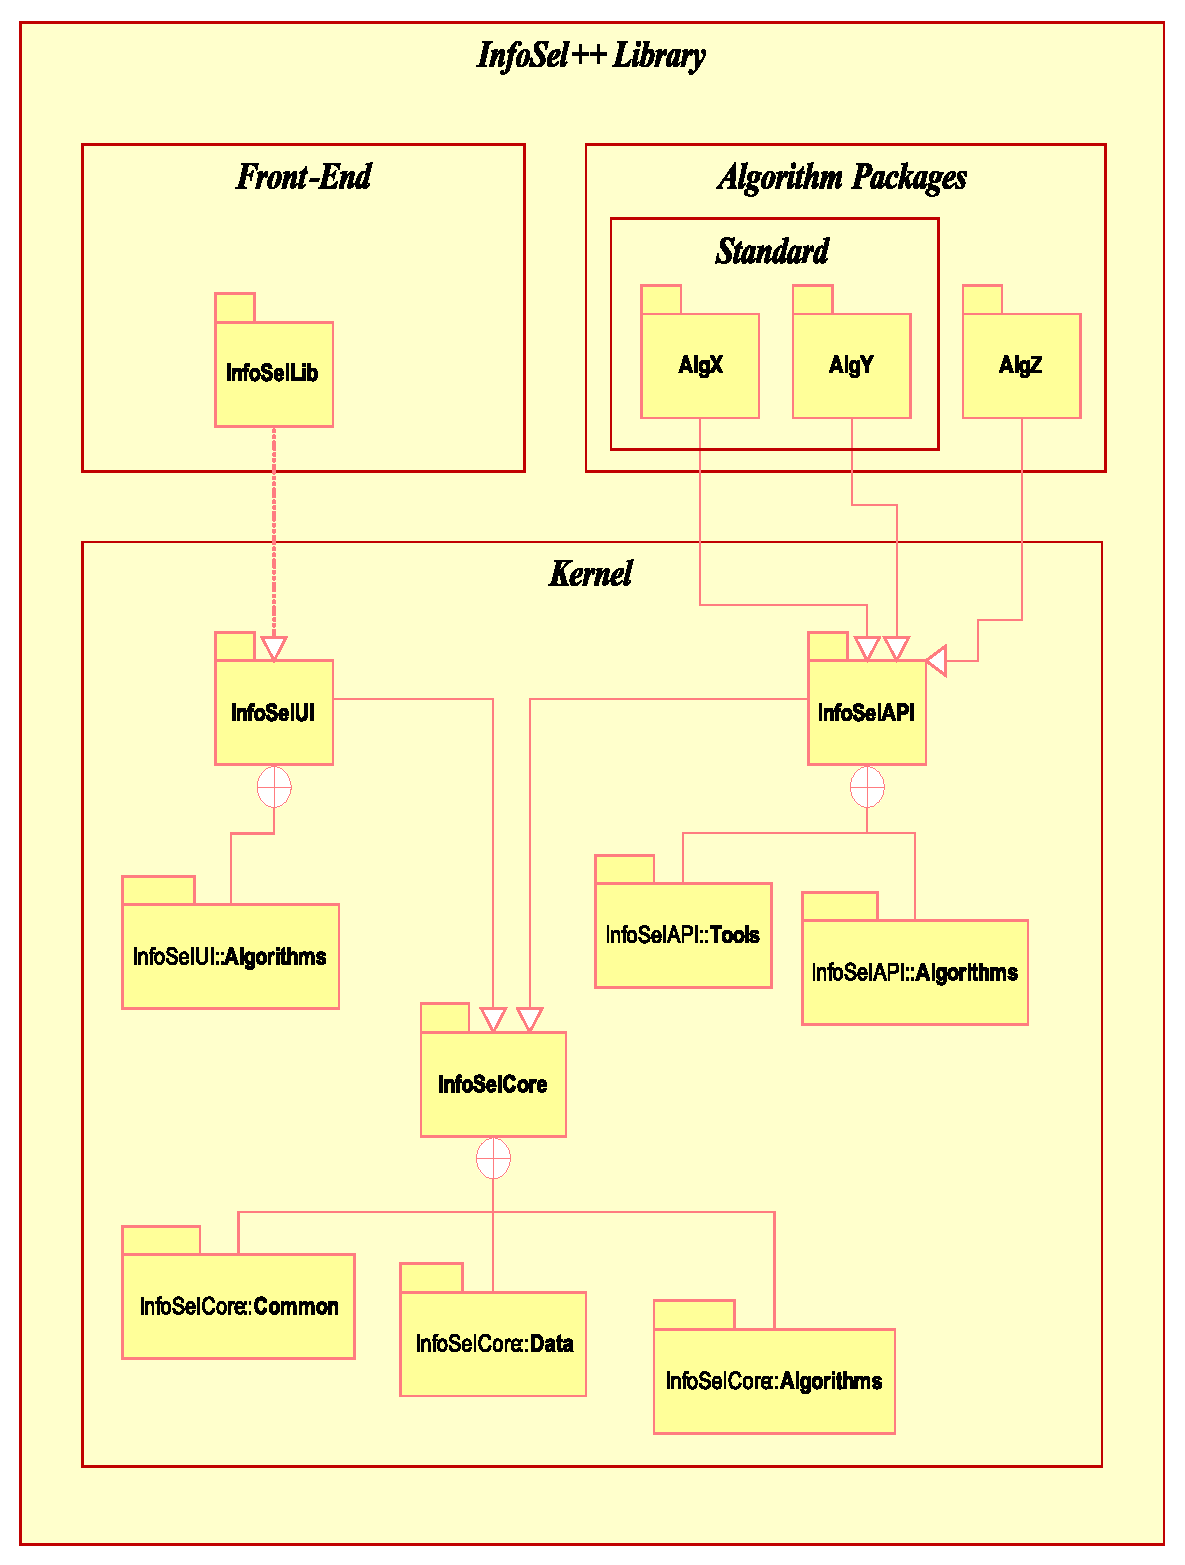
\includegraphics[width=3in]{./figs/Lib-mainstrukture.eps}
  \end{center}
  \label{piclibmainstrukture}
  \caption{\small Main architecture of library.}
\end{figure}

%\newpage
\begin{itemize}
\item InfoSelLib -- a module of front, high-level user interface libraries, the purpose of which is encapsulation 
                   of the internal structure of the library, 
                   with simultaneous access to most of the services offered by the low-level interface;
\item InfoSelUI -- a low-level user interface library module enabling direct access to the kernel library and execution of a feature selection process for selected algorithms;
\item InfoSelUI::Algorithms -- a submodule enabling the use of all feature selection algorithms (the ALGs collection), 
                 the classes and modules of which have been included and registered in the library;
\item InfoSelCore -- a central module of the kernel library responsible for the execution of major operations related to feature selection processes, 
                    such as reading data and input parameters, conversion of the input 
                    data to the appropriate structure in accordance with the adopted model, 
                   carrying out pre-processing of the input data, and execution of selected algorithms;
\item InfoSelCore::Common -- a submodule of useful elements for general purposes;
\item InfoSelCore::Data -- a submodule of classes representing main concepts associated with the input data structure, 
                 presented in the UML diagram in figure 4.3; % \ref{pic:lib-datastructure};
\item InfoSelCore::Algorithms -- a submodule of basic elements used in both the implementation and the utilization of the algorithms;
\item InfoSelAPI -- an API module enabling implementation of feature selection algorithms and their inclusion in the kernel library;
\item InfoSelAPI::Tools -- a submodule of tools which simplify writing the definition of an algorithm, presented in the UML diagrams in figure 4.4 and figure 4.5; % \ref{}
\item InfoSelAPI::Algorithms -- a submodule of elements enabling programmatic addition (registration) of classes and modules to the library;
\item AlgX, Algy, AlgZ -- modules X, Y, Z with feature selection algorithms added to the library.
\end{itemize}

The main library layer contains the kernel specific modules. The main role of the kernel is to read the data file and input parameters, 
to perform all processing on the initial data set, and to execute the requested feature selection algorithms. 
The most important data structures and other elements of the program are stored in a central module of the library, which is called 
InfoSelCore.  This module consists of 3 submodules: InfoSelCore::Common, InfoSelCore::Data, and InfoSelCore::Algorithms.
Another layer of the library is a collection of modules with selection algorithms defined (Algorithm Packages). 
Thanks to the open architecture of the library, each algorithm can be integrated as an independent, separately compiled module. 
Elective expansion of the library requires neither interference in the already existing code, nor its recompilation. 
This guarantees free and easy extensibility. For convenience, similar algorithms can be grouped into a single module. 
The name of the module may be the same as the name of a single algorithm or of the algorithm family. 
Module creation and implementation of its internal algorithms in the library environment require full access to the 
public elements of the library kernel. This is achieved using the InfoSelAPI module (API - Algorithm Programming Interface). 
Moreover, this module offers a number of additional elements grouped in submodules InfoSelAPI::Algorithms and InfoSelAPI::Tools, 
and intended
primarily for registering algorithms and writing their definitions. The API interface also introduces specific requirements for the implementation of algorithms in the source code of the module. For instance, each feature selection algorithm should
be represented in the form of a separate C++ class derived from the base class InfoSelCore::Algorithms::Algorithm. The content of the definition of the algorithm 
is stored in the form of virtual methods, also derived from the base class. 
Adoption of the object oriented model makes the overall library code clearer and more concise, comparable to mathematical notation. In particular, the extended object model has been adopted in the structure of the input data, where classes 
representing the main concepts of feature selection, such as input file, features and feature sets, space of subsets of features, 
and probability distribution, have been specified.

The execution of a complete feature selection process for the given input data and for the selected algorithms is done 
by selecting the appropriate user interface library.  The low-level interface, intended exclusively for use in the C++ code,
offers a module InfoSelUI (UI - User Interface). This module allows any given code direct access to the core elements of public libraries and collections registered in the algorithms library. 
This collection is located in the submodule InfoSelUI::Algorithms.  
The use of the library at a higher level, \ie, without direct reference to the kernel, 
is provided by the front layer of the library. 
This layer includes a series of high-level user interfaces, 
which make the majority of the low-level interface services available, while obscuring the InfoSelUI code library. 
The InfoSelLib module of the front layer contains the basic interfaces in the form of two classes: Script and Entry, 
both intended for use in the C++ code. The former class is a convenient-to-use interface library that provides easy connection 
between library and other system components, such as a command-line program with an interactive interface in the text mode, 
or a GUI type application. In addition, the Entry class allows the library to be used with other data processing software.
The class Script is a scripting interface, which allows the library to be used in batch mode.

%%%%%%%%%%%%%%%%%%%%%%%%%%%%%%%%%%%%%%
%  We done this to 03.31.2010
%%%%%%%%%%%%%%%%%%%%%%%%%%%%%%%%%%%%%%
%\vspace[*]{-3in}
\begin{figure}[!h] \label{pic:lib-generalelments}
  \begin{center}
    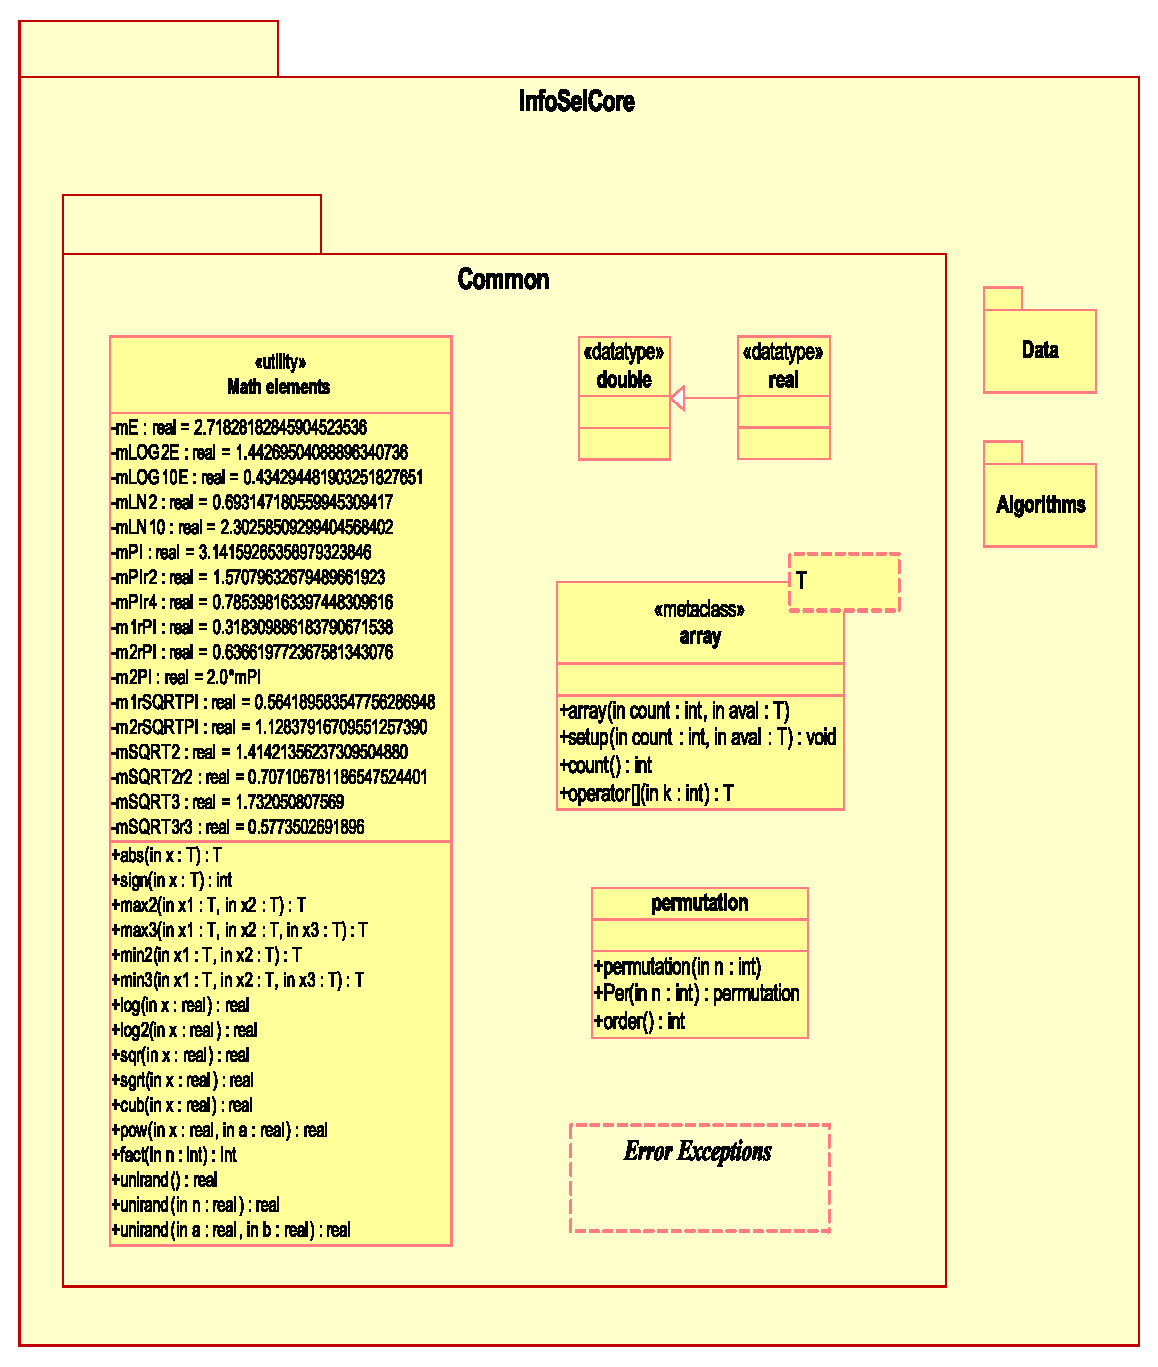
\includegraphics[height=4in,width=4in]{./figs/Lib-generalelements.eps}
  \end{center}
  \caption{\small General elements of library.}
\end{figure}

The general elements of the library listed below are a part of InfoSelCore namespace: 

\begin{itemize}
\item Math elements -- a collection of mathematical constants and functions which are commonly used in the library code;
\item array -- a class template representing any type of data arrays;
\item permutation -- a simple class representing permutation of integers of the n-th order;
\item double -- an equivalent of the C++ double type;
\item real -- an alias name for the double type;
\end{itemize}	

\begin{itemize}
\item xError -- a base exception covering all types of errors in the library;
\item xUnknownExn -- an exception representing unknown errors;
\item xToolError -- an exception for all errors related to the tools for algorithm implementation;
\item xInOutError -- an exception for all errors associated with the input/output operations;
\end{itemize}

Another part of the library consists of elements of the InfoSelCore::Data, which describes the algebraic elements of dataset.
All these elements and their definitions are as follows:

\begin{itemize}
\item datum -- a class representing a single (atomic) value of the input data;
\item datcolumn -- a class representing a column of data in the input file. Each column is a total aggregate of objects of class datum.
\item datvector -- a class representing a vector of data in the input file, each vector is a partial aggregate of objects of class datum;
\item datset -- a class representing a collection of all data read from the input file.
               The set is organized as a complete aggregate of datcolumn objects and 
               may also be formally treated as an aggregate of objects of class datvector;
\item subdatset -- a class representing a subset of the data set of partial aggregation;
\item datspace -- a class representing a space (set) of all data subsets. The space can be formally treated as an 
                 aggregate of subdatset objects;
\item datfile -- a class representing the input data file. The file is a total aggregate of datset objects and 
                is also the root of the object graph modeling the structure of the input data in the library.
%%%%%%%%%%%%%%%%%%%%%%%%%%%%%%%%%%%%%%%%%%%%%%
% Check 
%%%%%%%%%%%%%%%%%%%%%%%%%%%%%%%%%%%%%%%%%%%%%%
\item repfile -- a class representing the output file containing the report of the feature selection process 
                and the calculation results;
\end{itemize}

\begin{figure}[!hb] \label{pic:lib-datastructure}
  \begin{center}
     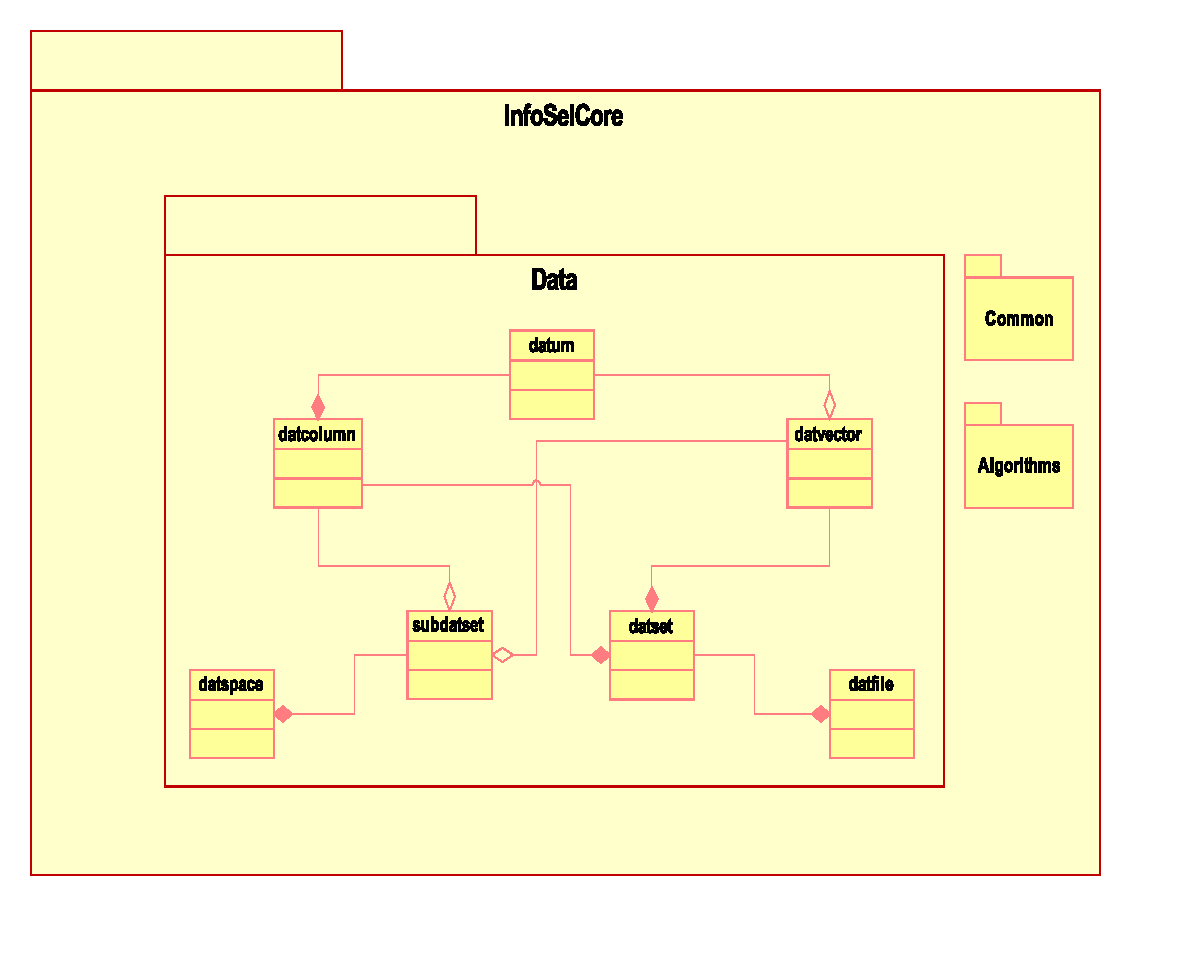
\includegraphics[height=4in,width=4in]{./figs/Lib-datastructure.eps}
   \end{center}
   \caption{\small Aggregate elements of input data.}
\end{figure}


\begin{itemize}
\item Algorithm - a base class of all registered classes of feature selection algorithms;
\item xAlgsError - exception errors associated with algorithms library;
\item xUnknownAlgorithm - an exception for unknown algorithm error;
\item Register - a class template used in the registration directive of an algorithm ALG class.
\end{itemize}

\begin{figure}[!hb] \label{pic:lib-tools}
   \begin{center}
     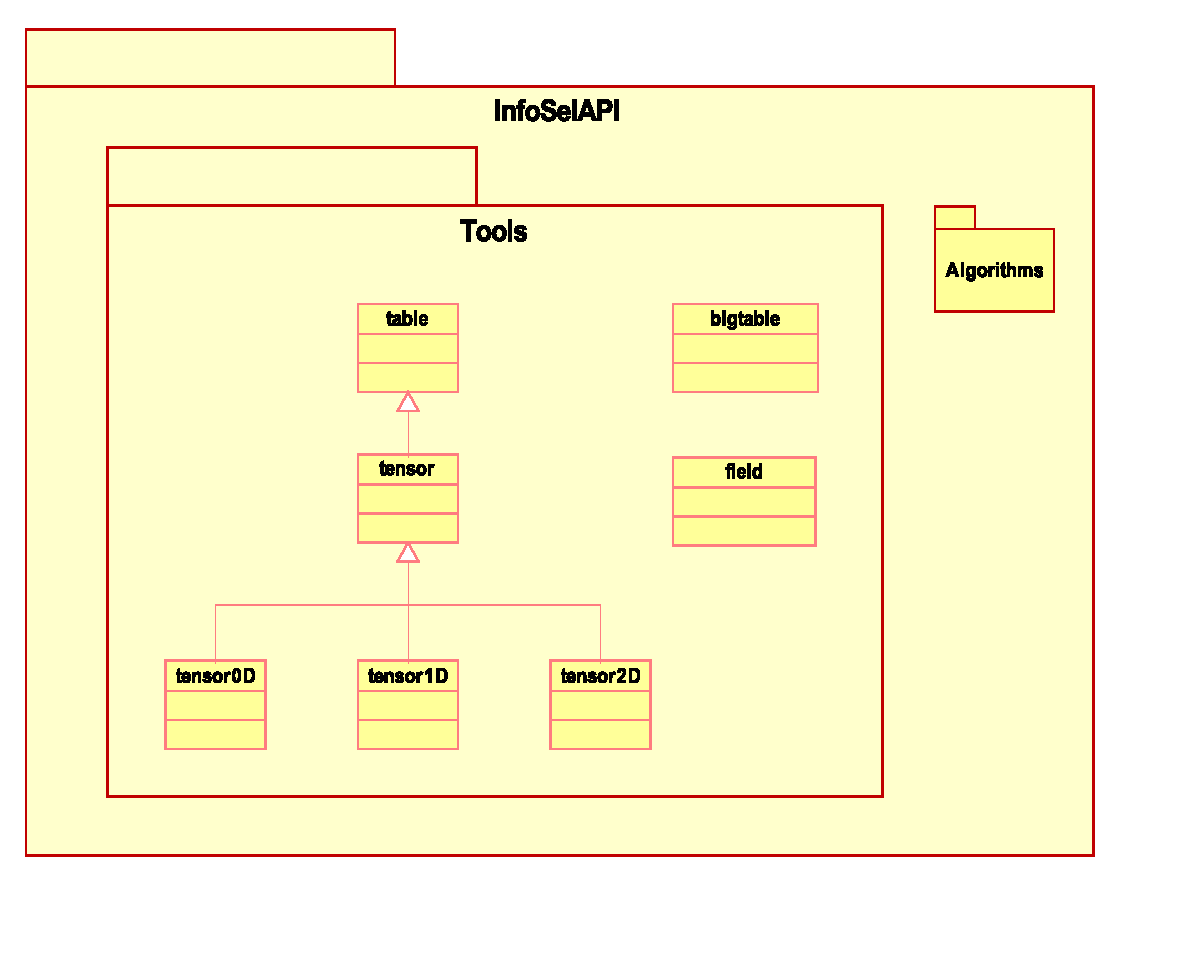
\includegraphics[width=4in]{./figs/Lib-tools.eps}
   \end{center}
   \caption{\small Basic classes used for algorithm implementation.}
\end{figure}

The last group lists the main elements included in InfoSelAPI:Tools namespace, which is
responsible for implementing the probability tables, distribution tables, and classes used for algorithm creation (implementation).

\begin{itemize}
\item table -- a multi-dimensional array of real-type numbers, used for storing the interim and final feature selection calculation results. For each dimension the table has a separate size identifying the size of a subarray;
\item tensor -- a multidimensional tensor created as an array of class table with fixed size for all dimensions;
\item tensor0D -- 0-dimensional tensor (single number);
\item tensor1D -- 1-dimensional tensor (vector of numbers);
\item tensor2D -- 2-dimensional (square matrix of numbers);
\end{itemize}

\begin{figure}[!b] \label{pic:lib-toolsb}
  \begin{center}
    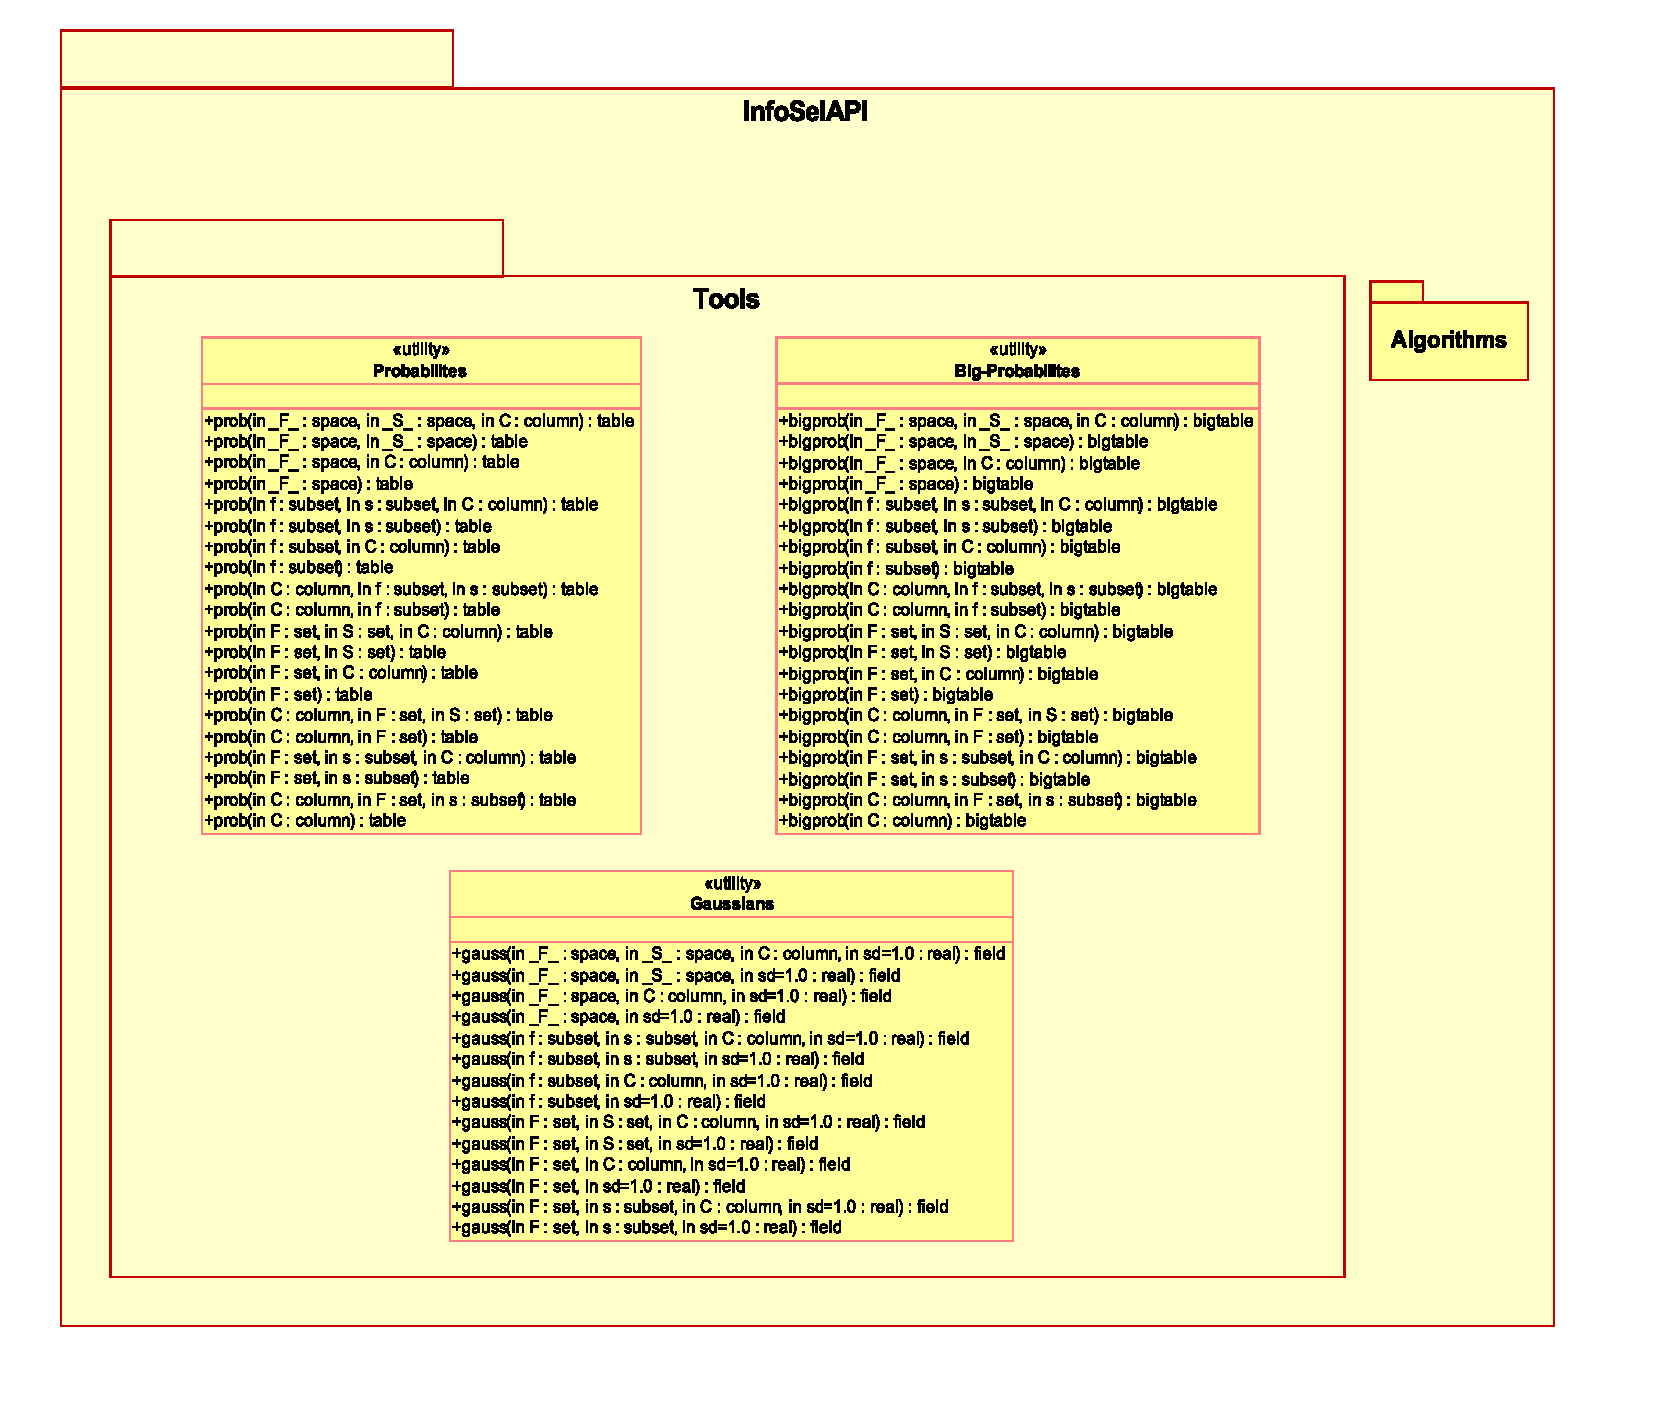
\includegraphics[width=4in]{./figs/Lib-toolsB.eps}
  \end{center}
  \caption{\small Details of basic classes used for algorithm implementation.}
\end{figure}


\begin{itemize}
\item BigTable -- a variant of a class table array, whose size/dimensionality can take large values. To avoid overloading the RAM memory, this structure was implemented using hashing techniques;
\item field -- a multidimensional continuous field whose values are arrays of class table.
\item Probabilities -- procedures that return an array of class table. Return arrays contain probability distribution of the input data, differentiated according to the type of data structures, imputed (passed) as arguments of procedure calls;
\item Big-Probabilities -- same procedures, as described above, except that return arrays are of class BigTable;
\item Gaussians -- same procedures as desribed above, returning an object of field type with the density probability distribution function of the input data smoothed with a Gaussian function;
\item ALGs -- a collection of objects of all included and registered classess of feature selection algorithms;
\item Entry -- a class representing the type of mandatory front interface, allowing easy linking with the other components of the system;
\item Algorithm -- a helper class representing a record with the description of a feature selection algorithm used in the interface Entry;
\item Script -- class representing the type of scripting front interface which allows the use of the library by a program running in batch mode.
\end{itemize}


%Infosel++ is a class library for development of feature selection algorithm based on probability distribution. Infosel++ is
%a cross-platform library. Version 1.01 has been released for Windows (Microsoft .NET compiler) and Linux (gcc 4.2) systems.

%Infosel++ include a library of general purpose classes, independent of machine learning, called InfoSelCore (InfoSelCore::Common).
%InfoSelCore::Comon classes include arrays, hash tables, math-elements and output/input streams, as well as some built-in mechanisms 
%for dealing with C++ initialization order, options, temporary generation and cleanup, as well as interrupt handling.

%The important concepts for feature selection provided by the library include point (element of column - datum), 
%column with data - feature (datcolumn),
%vector with data (datvector), dataset (datset), subset of features (subdatset), 
%data file (datfile) etc. (In parenthesis we have name of classes).

%In InfoSelAPI include several class and methods important for implementation of algorithm, such as table (bigtable - hash table), 
%tensor0D, tensor1D, tensor2D, temporary structure for storing a calculated value during a feature selection processing and method 
%related to calculation of probability distribution (one or multi-dimensional) called prob (bigprob).

%All implemented algorithm are stored and ordain automatically in special modules called 
%InfoSelUI:: Algorithms and InfoSelAPI::Algorithms, which allows create hybrid feature selection algorithm in automatic way.

%Programming with Infosel++ generally require little coding, simple example of source code for mutual 
%information ranking in next section.



%\include{./libstuctere}  % description of library structure
%\include{./libstuctere_it}


\section{Code Example} \label{sec:CodeExample}

A commonly used ranking in feature selection uses Mutual Information as a critical function, defined as 
a special case of Kullback-Leiber divergence: 
\begin{equation} \label{eq:kldiv}
D_{KL}(p(f,C) \| p(f)p(C))\;=\;MI(f,C)\;=\;\sum_{i,k\in C}p(f_i,c_k)\log \frac{p(f_i,c_k)}{p(c_k)p(f_i)}
\end{equation}
or uses entropy for the feature and the vector class, and joint entropy between feature and class: 
\begin{eqnarray} \label{eq:entropies}
MI(f,C) &=& H(f)+H(C)-H(f,C) \\
        &=& -\sum_{i} p(f_i) \log{p(f_i)} -\sum_{k\in C} p(c_k) \log{p(c_k)} + \sum_{i,k\in C} p(f_i,c_k) \log{p(f_i,c_k)} \nonumber
\end{eqnarray}

Implementation of ranking based on Mutual Information with implemented algebraic structure in the Infosel++ library:

{\scriptsize
\begin{verbatim}
 1.  const int vnt=variant();
 2.  const real delta=delta_;

 3.  datspace _F_(F,1);
 4.  datspace _S_(S,1);

 5.  table P_FC = prob(_F_,C);
 6.  table P_F = prob(_F_);
 7.  table P_C = prob(C);

 8.  table H_FC = -sum(sum(P_FC*log2(P_FC)));
 9.  table H_F = -sum(P_F*log2(P_F));
 10. table H_C = -sum(P_C*log2(P_C));

 11. vector MI_FC = H_C + H_F - H_FC;

 12. rep.log() << "Entropy H(F,C) = " << H_FC << endl;
 13. rep.log() << "Entropy H(F) = " << H_F << endl;
 14. rep.log() << "Entropy H(C) = " << H_C << endl;
 15. rep.log() << "MI-coefficient MI(F,C) = " << sorted << MI_FC << endl;

 16. // vector MI_FC = sum(sum( P_FC*log2(P_FC/(P_F^P_C)) ));
 17. // rep.log() << "Mutual information MI(F,C) = " << sorted << MI_FC << endl;

 18. S.reversion(true);

 19. if (vnt==vRank){
 20.  subdatset f = argmax(_F_, MI_FC );
 21.   while (!f.isnil()) {
 22.   F-=f;
 23.   S+=f;
 24.    if (completed(file)) break; 
 25.    f = argmax(_F_, MI_FC);
 26.    if (MI_FC(f) <= delta ) break;
 27.   }
 28. }
\end{verbatim}
}

The first two lines define two parameters. The first is "vnt", which represents a search method, in our case, a ranking, 
the simplest kind of search method; the second parameter, "delta", is a cut-off value for finishing a ranking.
Below this value all features will be rejected (default value 0.05). 
The next two lines (3. and 4.) represent two subsets, one initial subset with all features and a second one where features 
are stored after fulfilling the condition of our algorithm. The stored feature is deleted from the initial subset of features.
%The next three lines (5-7) define tables with probabilities as well as joint probability between features and class for all features 
%in subset F, and for features F and class C. 
The next three lines (5-7) define tables of joint probability between features and class for all features 
in subset F as well as probabilities of features in subset F and class C, respectively.
Lines 8-10 represent entropies for the subset of features, class, and joint entropy between class and
features (defined in eq. \ref{eq:entropies}). In line 11 we have defined Mutual Information as a function of entropies 
(eq. \ref{eq:entropies}). This line is equivalent to line 16 where we show the possibility of using Mutual 
Information defined by equation \ref{eq:kldiv}. The sole function of line 17 is to report values of Mutual Information.

%
Lines 12-15 represent reports about calculated entropies and mutual information. Line 18 describes the direction of sorting of features
based on the ranking function. The main algorithm starts at line 20, where we initiate an algorithm by selecting the feature 
with the maximum value of MI.
Lines 21-27 represent main while loop, which is finished when subspace F is empty or a maximal value of MI in subset F is below the delta value (line 26).

In case of the Battiti \cite{Battiti1994} algorithm, where the evaluated (maximized) formula is presented in the first row of table 3.1. % \ref{tab:diffschems}. 
We need to add (modify) several lines but not the reporting line (line 12-16 in previous list of code). Firstly, add the line with mutual information (1a). 
Then modify line 25 and delete line 26. The important changes to the previous code are listed below. This is an implementation of the Battiti algorithm:

{\scriptsize
\begin{verbatim}

 1a. matrix MI_FF = sum(sum( P_FF*log2(P_FF/((P_F^P_F)*Per(4)(0,2,1,3))) ));
 
 2a. rep.log() << "Mutual information MI(F,C) = " << sorted << MI_FC << endl;
 3a. rep.log() << "Mutual information MI(F,F) = " << MI_FF << endl;

 4a.  S.reversion(true);

 5a.  subdatset f = argmax(_F_, MI_FC );
 6a.  while (!f.isnil()) {
 7a.   F-=f;
 8a.   S+=f;
 9a.   if (completed(file)) break;
 10a.    f = argmax(_F_, MI_FC-beta*sum(_S_,*MI_FF) );
 11a.  }
 12a. }
\end{verbatim}
}

These two simple examples show that the Infosel++ interface can be a useful framework for developers for creating and testing 
algorithms based on probability distribution.

%\include{./libexample}   % description of simple source code



\appendix


\chapter{Project directory structure} \label{sec:InfoselDirStr}

\begin{scriptsize}
 \begin{verbatim}
   build                :  project distribution building
      GNUC++            :  building with any GNU C++ compiler
        out             :  intermediate object files
      VisualC++         :  building with the Microsoft Visual C++ ver.8
   dist                 :  project distribution directory
      bin               :  executable files
      lib               :  library/archive files
      include           :  C++ include files
      doc               :  documentation files
      src               :  sample source files
      make              :  sample make files
        out             :  intermediate object files
      test              :  command files for testing programs
      work              :  command files for running programs
   prj                  :  main project directory
      library           :  source files of main library
        kernel          :  kernel source files
        frontend        :  front-end source files
      libpacks          :  standard package files with algorithm implementation
      libapps           :  source files of library applications
        stdcon          :  standard console source files
        samples         :  samples source files
      libtests          :  source files of library tests for integral 
                                        (all) and units: API, UI and front-end
      libdocs           :  source files of library documentation
        manual          :  manual source files
        design          :  library design documentation
        examples        :  example files for data, scripts and algorithm packs
        manual          :  manual source files
        reference       :  DOXYGEN reference files
 \end{verbatim}
\end{scriptsize}

%\begin{postscript}
%\begin{directory}{\url{infosel_lib/}}
%  \file{\begin{directory}{\url{build/}}
%\end{postscript}
%\include{./libstr}


\chapter{Concise dictionary} \label{sec:InfoselDefintion}

Below we can find several definitions and concepts important to the understanding of the tutorial ({\it cf.} \cite{HuanLiu2004}). 

F is a symbolical representation of a full set of features , where $F_i$ is a one feature, and $S_i = F / \{F_i \}.$ 

\begin{definition}{\bf (Strong relevance)} A feature $F_i$ is strongly relevant if
\end{definition}
\begin{equation}
         \mathbf{P} ( C|F_{i}, S_{i} ) \neq \mathbf{P} ( C|S_{i} ) \nonumber
\end{equation}

\begin{definition}{\bf (Weak relevance)} A feature $F_i$ is weakly relevant if
\end{definition}
\begin{equation} 
       \mathbf{P} ( C|F_{i}, S_{i} ) = \mathbf{P} ( C|S_{i} ) \;\;and\;\; \nonumber
\end{equation}
\begin{equation} 
         \exists S^{'}_{i} \subset S, \; such\;\; as\; \mathbf{P} ( C|F_{i}, S^{'}_{i} )
         \neq \mathbf{P} ( C|S^{'}_{i} ) \nonumber
\end{equation}

\begin{corollary}{\bf (Irrelevance)} A feature $F_i$ is irrelevant if\end{corollary}
\begin{equation}
       \forall S^{'}_{i} \subseteq S, \mathbf{P} ( C|F_{i}, S^{'}_{i} ) = \mathbf{P} ( C|S^{'}_{i} )
\end{equation}
\begin{definition}{\bf (Markov Blanket)} Given a feature $F_i$, let $M_{i} \subseteq F ( F_{i} not \in M_{i} ) $, $M_{i}$
 is said to be a Markov Blanket for $F_i$ if
\end{definition}
\begin{equation}
         \mathbf{P} ( F - M_{i} - \{ F_{i} \} , C | F_{i}, M_{i}) \;=\;
         \mathbf{P} ( F - M_{i} - \{ F_{i} \} , C | M_{i} )
\end{equation}

\begin{definition}{\bf (Redundant feature)} Let G be the current set of features. A feature is redundant and
hence should be removed from G if it is weakly relevant and has a Markov Blanket $M_i$ within G .
\end{definition}
\begin{definition}{\bf (C-correlation)} The correlation between any feature $F_i$ and class C is called C-correlation,
denoted by $SUC_{i,c}$ \end{definition}
\begin{definition}{\bf (F-correlation)} The correlation between any pair of features $F_i$ and $F_j$ ($i \neq j$) is called
F-correlation, denoted by $SUC_{i,j}$.
\end{definition}
\begin{definition}{\bf (Approximate Markov Blanket)} For two relevant features $F_i$ and $F_j$ ($i \neq j$), $F_j$ forms
an approximate Markov Blanket for $F_i$ if $ SUC_{i,c} \geq SUC_{i,c}$ and $ SUC_{i,j} \geq SUC_{i,c}$ .\end{definition}
\begin{definition}{\bf (Predominant feature)} A relevant feature is predominant if it does not have any
approximate Markov Blanket in the current set.\end{definition}
%\include{./defintions}


\chapter{Command line parameters} \label{sec:Infoselparam}
Synatx of parameters recognized by infosel++ aplication:
\begin{scriptsize}
 \begin{verbatim}
  -h|help [file_name]
    Displays this help info or writes it to a given file.

  -s|scr|script file_name
    Performs processing of a given script file.

  -in|input|data file_name
    Sets up input data file.

  -out|output|report file_name
    Sets up output report file.

  -p|prec|precision real_val
    Sets up real data precision.

  -pm|pmeth|partition meth_name|meth_name(val_list)
    Sets up data partition method.

  -cp|cpos|classpos int_val
    Sets up classes column position.

  -lc|lastc|classislast bool_val
    Sets up a flag whether classes column is last.

  -e|excl|excluded str_list
    Sets up labels for excluded classes.

  -ne|note|notexcluded str_list
    Sets up labels for non excluded classes.

  -m|merg|merged str_list
    Sets up labels for merged classes.

  -nm|notm|notmerged str_list
    Sets up labels for non merged classes.

  -exe|exec|exeselalg alg_tag|alg_tag(val_list)
    Executes a given selection algorithm.

  -execall
    Executes all selection algorithms.

  -silent
    Perform processing without displaying output info.

  -verbose
    Performs processing displaying more output info.

  -break
    Breaks processing commands.
  \end{verbatim}
\end{scriptsize}

%\include{./infparameters}

%\bibliographystyle{plain}
%\bibliographystyle{ama}
\bibliographystyle{ieeetr}
\bibliography{infosel}

\end{document}

